\documentclass[conference]{IEEEtran}
\IEEEoverridecommandlockouts
% The preceding line is only needed to identify funding in the first footnote. If that is unneeded, please comment it out.
\usepackage{cite}
\usepackage{amsmath,amssymb,amsfonts}
\usepackage{algorithmic}
\usepackage{graphicx}
\usepackage{textcomp}
\usepackage{xcolor}
\usepackage{float}
\usepackage{listings}
\usepackage{amsmath}
\usepackage{subcaption}
\usepackage{tikz}
\usepackage{pgfplots}
\pgfplotsset{compat=1.17}
\usepackage{caption}
\usepackage{booktabs}
\usepackage{multirow}
\usepackage{siunitx}
\usepackage{url}
\def\BibTeX{{\rm B\kern-.05em{\sc i\kern-.025em b}\kern-.08em
    T\kern-.1667em\lower.7ex\hbox{E}\kern-.125emX}}
\begin{document}

\title{Credit Card Fraud Detection\\}

\author{\IEEEauthorblockN{1\textsuperscript{st} André Almeida Oliveira}
\IEEEauthorblockA{\textit{Tópicos de Aprendizagem Automática 23/24} \\
\textit{
DETI
}\\
\textit{
University of Aveiro
}\\
Aveiro, Portugal \\
andreaoliveira@ua.pt}
\and
\IEEEauthorblockN{2\textsuperscript{nd} Duarte Carvalho da Cruz}
\IEEEauthorblockA{\textit{Tópicos de Aprendizagem Automática 23/24} \\
\textit{DETI}\\
\textit{University of Aveiro}\\
Aveiro, Portugal \\
duarteccruz@ua.pt}
}

\maketitle

\begin{abstract}
Credit card fraud remains a pervasive issue, causing substantial financial losses for individuals and institutions worldwide. This project aims to develop a robust system for automatic fraudulent transaction detection using a comprehensive dataset of 284,807 transactions. Each transaction record includes 29 transformed data columns essential for analysis. Due to the nature of fraudulent activity, the dataset exhibits significant class imbalance, posing a specific challenge for machine learning models. To mitigate this, a range of potential algorithms, including those specifically designed for imbalanced datasets, will be explored and evaluated.  Performance metrics tailored to the imbalanced context, such as F1-score and weighted accuracy, will be used to optimize the system's effectiveness in a real-world setting. This work has the potential to contribute valuable insights to the ongoing efforts in mitigating credit card fraud.
\end{abstract}

\section{Introduction}
The rise of digital commerce has revolutionized the way we conduct transactions, but it has also opened doors for sophisticated financial crimes like credit card fraud. This pervasive issue erodes trust in electronic payment systems, leading to substantial losses for individuals, businesses, and financial institutions globally. Recognizing the severity of this problem, we chose to focus our "Tópicos de Aprendizagem Automática" (Topics of Automated Learning) project at the Universidade de Aveiro on the development of a machine learning-driven solution for credit card fraud detection. We were drawn to the challenge of working with real-world data to create a system that could potentially safeguard consumers and businesses in the digital economy.

The potential applications of a robust fraud detection system extend far beyond the classroom. Such tools could be integrated into payment platforms, providing real-time alerts and reducing the financial damage caused by fraudulent activity. As studenst exploring the frontiers of artificial intelligence, this project offered a unique opportunity to apply our developing skills, gain insights into algorithm design, and contribute to tackling a problem with tangible consequences. This report delves into the strategies explored, the challenges encountered, and the lessons learned throughout our exploration of machine learning for credit card fraud detection.

\section{State of the Art}

In the realm of credit card fraud detection, researchers have explored various machine learning techniques to tackle the challenges posed by fraudulent activities. Traditional models such as Logistic Regression, Decision Trees, Random Forests, and Support Vector Machines (SVM) have been extensively employed due to their interpretability and effectiveness, especially when dealing with smaller datasets \cite{b4}. Conversely, neural networks, including Convolutional Neural Networks (CNNs) and Recurrent Neural Networks (RNNs), have emerged as powerful tools for capturing intricate patterns within vast transaction datasets, albeit at the expense of increased computational resources \cite{b14}. Ensemble methods, which combine predictions from multiple models, and hybrid techniques, incorporating feature engineering, anomaly detection, and autoencoders, have also contributed to improving detection accuracy.

A critical aspect of fraud detection lies in addressing class imbalance within datasets, where fraudulent transactions are typically rare. Techniques such as oversampling (e.g., SMOTE), undersampling, and cost-sensitive learning have been employed to alleviate bias towards the majority class \cite{b13}. Furthermore, algorithms inherently robust to class imbalance have been developed. Evaluation metrics beyond standard accuracy, including recall (sensitivity), precision, F1-score, and AUC-ROC, are imperative for providing insightful assessments of model performance in real-world fraud detection scenarios.

Recent advancements in fraud detection have seen a shift towards enhancing model explainability to foster trust in complex predictions. Additionally, there's a growing interest in exploring unsupervised and semi-supervised learning techniques, particularly beneficial when labeled data is limited or when fraud patterns are less well-defined.

The provided notebooks exemplify the efficacy of both traditional machine learning and neural network approaches in tackling credit card fraud detection \cite{b2, b3}. To excel in this domain, it is imperative to explore a diverse range of model families, integrate techniques tailored to address class imbalance, and adopt a comprehensive evaluation strategy prioritizing real-world performance metrics.

In addition to established approaches and recent trends, it's crucial to consider insights and findings from existing literature on credit card fraud detection.

One notable work \cite{b4} offers a comprehensive overview of the challenges and methodologies employed in fraud detection, providing valuable insights into the landscape of fraud detection techniques. This source sheds light on the effectiveness of classical machine learning models and the importance of feature engineering in detecting fraudulent activities.

Another relevant study \cite{b5} introduces a novel approach using Spatio-Temporal Attention-Based Neural Networks for credit card fraud detection. This work explores the application of advanced neural network architectures, specifically designed to capture spatio-temporal patterns inherent in transaction data. Such methods represent the forefront of research in leveraging deep learning for fraud detection tasks.

Furthermore, research published in \cite{b6} delves into the intricacies of fraud detection algorithms, offering insights into the limitations of existing methods and proposing novel solutions to enhance detection accuracy and efficiency. This study contributes to the ongoing discourse on the development of robust fraud detection systems.

Lastly, \cite{b7} presents practical applications of machine learning techniques in fraud detection, highlighting the importance of real-world implementation and performance evaluation. This work provides valuable case studies and empirical evidence of the effectiveness of machine learning algorithms in detecting fraudulent transactions.

By incorporating insights from these literature sources, we gain a comprehensive understanding of the challenges, methodologies, and advancements in credit card fraud detection, which informs our approach in developing effective fraud detection systems.

\section{Dataset Analysis}
\subsection{Dataset Description}\label{AA}
The analysis conducted in this project draws upon a dataset comprising a total of 284,807 transaction examples, which can be accessed through the provided link [1]. Among these transactions, the majority, totaling 284,315 instances, are categorized as normal, while a smaller subset of 492 instances are identified as fraudulent.

Each transaction within this dataset is represented by 31 columns, encompassing various attributes such as Time, V1 to V28, Amount, and Class. The initial 30 columns serve as features, with the majority adopting a naming convention utilizing the syntax Vnumber. Due to security considerations, many of these feature values are anonymized or transformed; for instance, while the cardholder's name may be represented as text, other values are converted into decimal numeric formats.

The final column, denoted as "Class," serves as the pivotal indicator of a transaction's legitimacy, where a value of "0" signifies a normal transaction and "1" indicates a fraudulent one.

\begin{figure}[htbp]
\centering
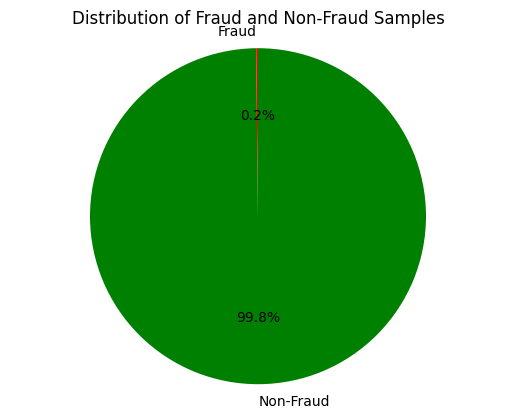
\includegraphics[width=0.5\textwidth]{images/fraudvsnonfraud1.png}
\caption{Distribution of Fraud and Non-Fraud Samples}
\label{fig}
\end{figure}
\begin{figure}
    \centering
    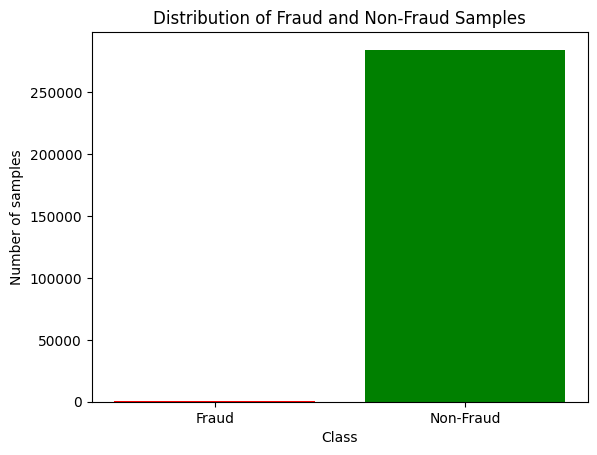
\includegraphics[width=1\linewidth]{images/fraudvsnonfraud2.png}
    \caption{Distribution of Fraud and Non-Fraud Samples}
    \label{fig:enter-label}
\end{figure}

As depicted in Figure 1 and Figure 2, the dataset exhibits a significant class imbalance, with a disproportionately larger number of non-fraudulent transactions compared to fraudulent ones. Specifically, non-fraudulent cases dominate the dataset, constituting approximately 99.83 \% of all transactions. Consequently, the proportion of fraudulent cases is exceedingly low, accounting for only about 0.17\% of the entire dataset.

This skew towards non-fraudulent cases presents a notable challenge in developing an effective classifier. The imbalance may lead the classifier to prioritize the identification of normal transactions, potentially misclassifying fraudulent transactions as normal. However, in the context of this study, the priority lies in minimizing false negatives, i.e., correctly identifying non-fraudulent transactions as fraudulent, rather than vice versa.


\subsection{Dataset Balancing}\label{DB}

\begin{figure}[H]
    \centering
    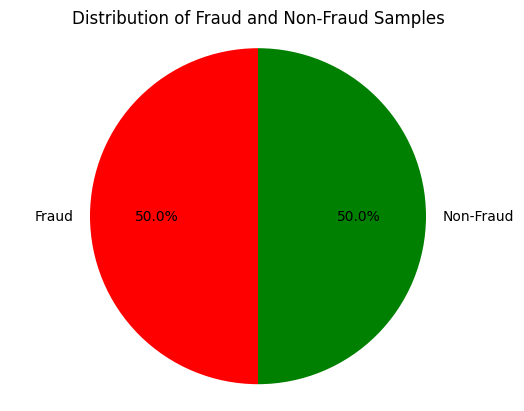
\includegraphics[width=1\linewidth]{images/subsamplepie.png}
    \caption{Balanced Data}
    \label{fig:enter-label1}
\end{figure}

In order to address the challenge highlighted in the previous section, a decision was made to sub-sample the dataset. But what exactly does this entail? Essentially, it involves adjusting the dataset to achieve balance. In this scenario, the aim is to create a fully balanced dataset with an equal proportion of fraudulent and non-fraudulent transactions, essentially a 50/50 split. By doing so, the issue of the classifier misclassifying results becomes less severe compared to if this balancing technique were not implemented.

As depicted in the image above and below (Fig 3. and 4.), the dataset now contains an equal number of fraudulent and non-fraudulent transactions.

\begin{figure}[H]
    \centering
    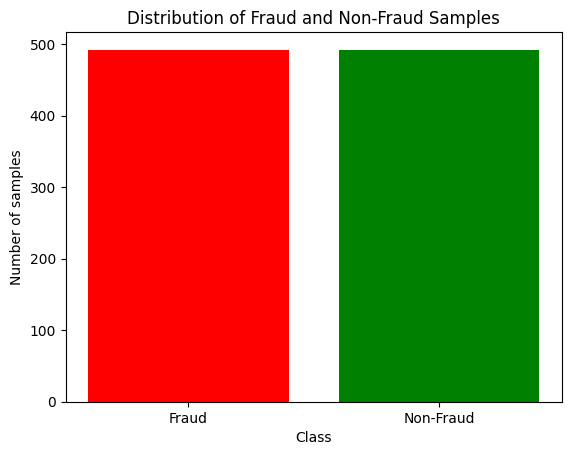
\includegraphics[width=1\linewidth]{images/subsamplingraph.png}
    \caption{Balanced data}
    \label{fig:enter-label2}
\end{figure}

\subsection{Normalization of the features}

Normalization of the data is still necessary. This step is crucial because certain features within the dataset may have significantly higher values compared to others. As a result, these features could disproportionately influence the outcome, skewing the analysis. To ensure that all features contribute equally to the analysis, normalization is performed.

In the code, the StandardScaler function from the sklearn.preprocessing module is utilized for normalization. According to its documentation, StandardScaler standardizes features by subtracting the mean and scaling them to unit variance.

\lstset{
    language=Python, % Linguagem do código
    backgroundcolor=\color{white}, % Cor de fundo
    basicstyle=\footnotesize, % Tamanho da fonte do código
    breaklines=true, % Quebra de linha automática
    captionpos=b, % Posição da legenda abaixo do código
    frame=single, % Adiciona uma borda ao redor do código
    numbers=left, % Exibe números de linha à esquerda
    numbersep=5pt, % Espaçamento entre os números de linha e o código
    numberstyle=\tiny\color{gray}, % Estilo dos números de linha
    showstringspaces=false, % Não destacar espaços em strings
    keywordstyle=\color{blue}, % Estilo das palavras-chave
    commentstyle=\color{green!40!black}, % Estilo dos comentários
    stringstyle=\color{red}, % Estilo das strings
}
\begin{lstlisting}
# Using the StandardScaler to normalize the data
from sklearn.preprocessing import StandardScaler

X = StandardScaler().fit_transform(X)
X = pd.DataFrame(X, columns=features)

data = pd.concat([data[features], data[label_column]], axis=1)
\end{lstlisting}


\subsection{Feature Analysis}

Given the extensive range of characteristics within the dataset, our aim was to assess the comparability of feature values across both fraudulent and non-fraudulent transactions. This evaluation was pivotal in identifying attributes that could offer stronger evidence of fraudulent activity. To achieve this, we generated bar graphs for each feature to discern which exhibited a higher degree of variation. A greater diversity in values suggested heightened relevance of a feature, potentially enhancing the effectiveness of our classifier within such environments.


\begin{figure}[H]
    \centering
    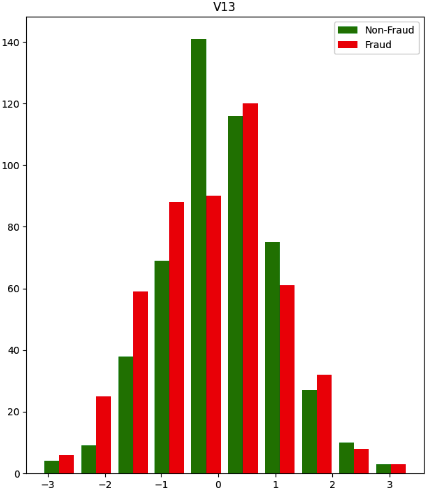
\includegraphics[width=1\linewidth]{images/feature13histogram.png}
    \caption{Example 1 of a bad feature (V13)}
    \label{fig:enter-label}
\end{figure}

\begin{figure}[H]
    \centering
    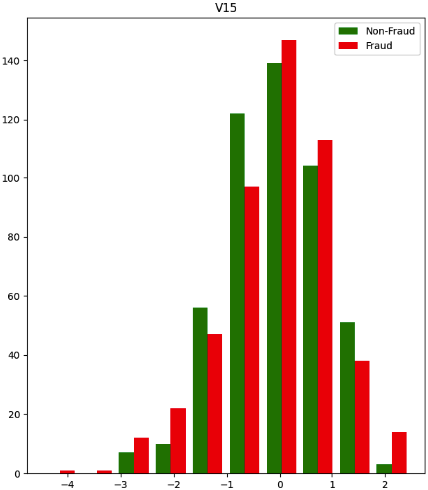
\includegraphics[width=1\linewidth]{images/feature15histogram.png}
    \caption{Example 2 of a bad feature (V15)}
    \label{fig:enter-label}
\end{figure}


Upon scrutinizing the graphical representation provided in the figures above, a nuanced understanding emerges regarding the potential influence of features V13, V15 on the detection of fraudulent transactions within the Credit Card Fraud Detection dataset. Notably, the comparative analysis of bar distributions across both fraudulent and non-fraudulent instances sheds light on the discriminatory capacity of these features.

Despite initial expectations, the observed consistency in bar patterns for varying attribute values across fraudulent and non-fraudulent transactions indicates a limited discriminatory power of features V13 and V15. This suggests that these particular attributes may not offer substantial insight or discriminatory leverage in distinguishing between fraudulent and legitimate transactions.

Furthermore, the near-identical nature of bar distributions implies that the behaviors captured by features V13 and V15 do not significantly deviate between fraudulent and non-fraudulent instances. Consequently, relying solely on these features for fraud detection may lead to suboptimal performance, as they may fail to capture the nuanced differences indicative of fraudulent activity.

In essence, the graphical analysis underscores the importance of discerning feature relevance in the context of fraud detection. While features V13 and V15 exhibit consistency across transaction types, further exploration of alternate features with greater discriminatory power may be warranted to enhance the efficacy of fraud detection algorithms. This iterative process of feature selection and refinement is crucial for developing robust and reliable fraud detection systems capable of accurately identifying fraudulent activities amidst the complexities of real-world transaction data.

\begin{figure}[H]
    \centering
    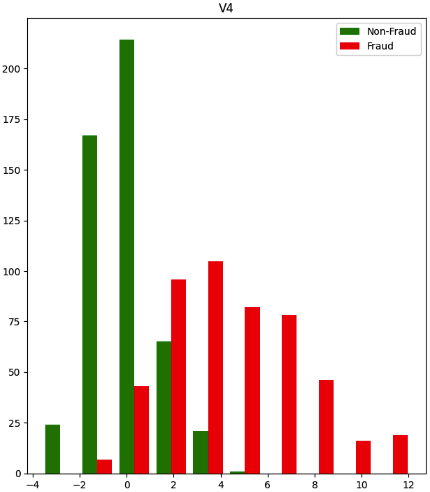
\includegraphics[width=1\linewidth]{images/feature4histogram.png}
    \caption{Example 1 of a good feature (V4)}
    \label{fig:enter-label}
\end{figure}

\begin{figure}[H]
    \centering
    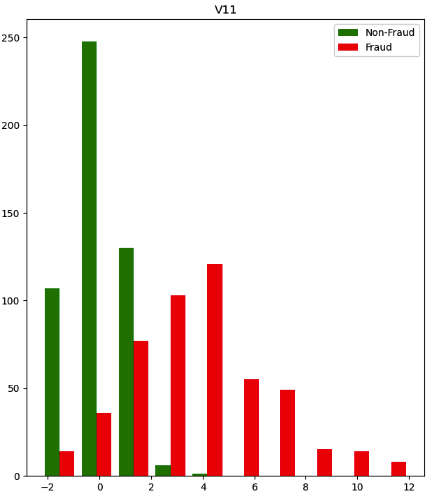
\includegraphics[width=1\linewidth]{images/feature11histogram.png}
    \caption{Example 2 of a good feature (V11)}
    \label{fig:enter-label}
\end{figure}

Going further in the investigation, Figs 7 and 8 offers a stark contrast to the observations made in Figs 5 and 6. Notably, the positioning of green and red bars distinctly differs within the graph. Particularly, when examining feature V11, a notable discrepancy arises: while occurrences of the value 0 are scarce in fraud transactions, they are abundant in normal instances. This discrepancy prompts a deeper consideration of the significance of features V4 and V11, suggesting that their values are more susceptible to alteration in the presence of fraudulent activity.

Thus, an informed analysis infers that these features may exhibit pronounced variations in response to fraudulent transactions. Consequently, delving into the intricacies of these features may yield more promising results than analyzing the broader set of 30 features available.


Exploring our dataset further, we employ a correlation matrix to gain insights into the relationships between different features. This analytical tool proves valuable in discerning which characteristics tend to be more predictive of fraudulent activities.

Our anticipation is that the features identified as significant indicators in this phase align closely, if not entirely, with those identified previously. Thus, we focus solely on creating a correlation matrix for the subsampled dataset. This approach allows us to underscore the significance of subsampling in refining our analysis and highlighting the pivotal role it plays in elucidating the underlying patterns and relationships within the data.

\begin{figure}
    \centering
    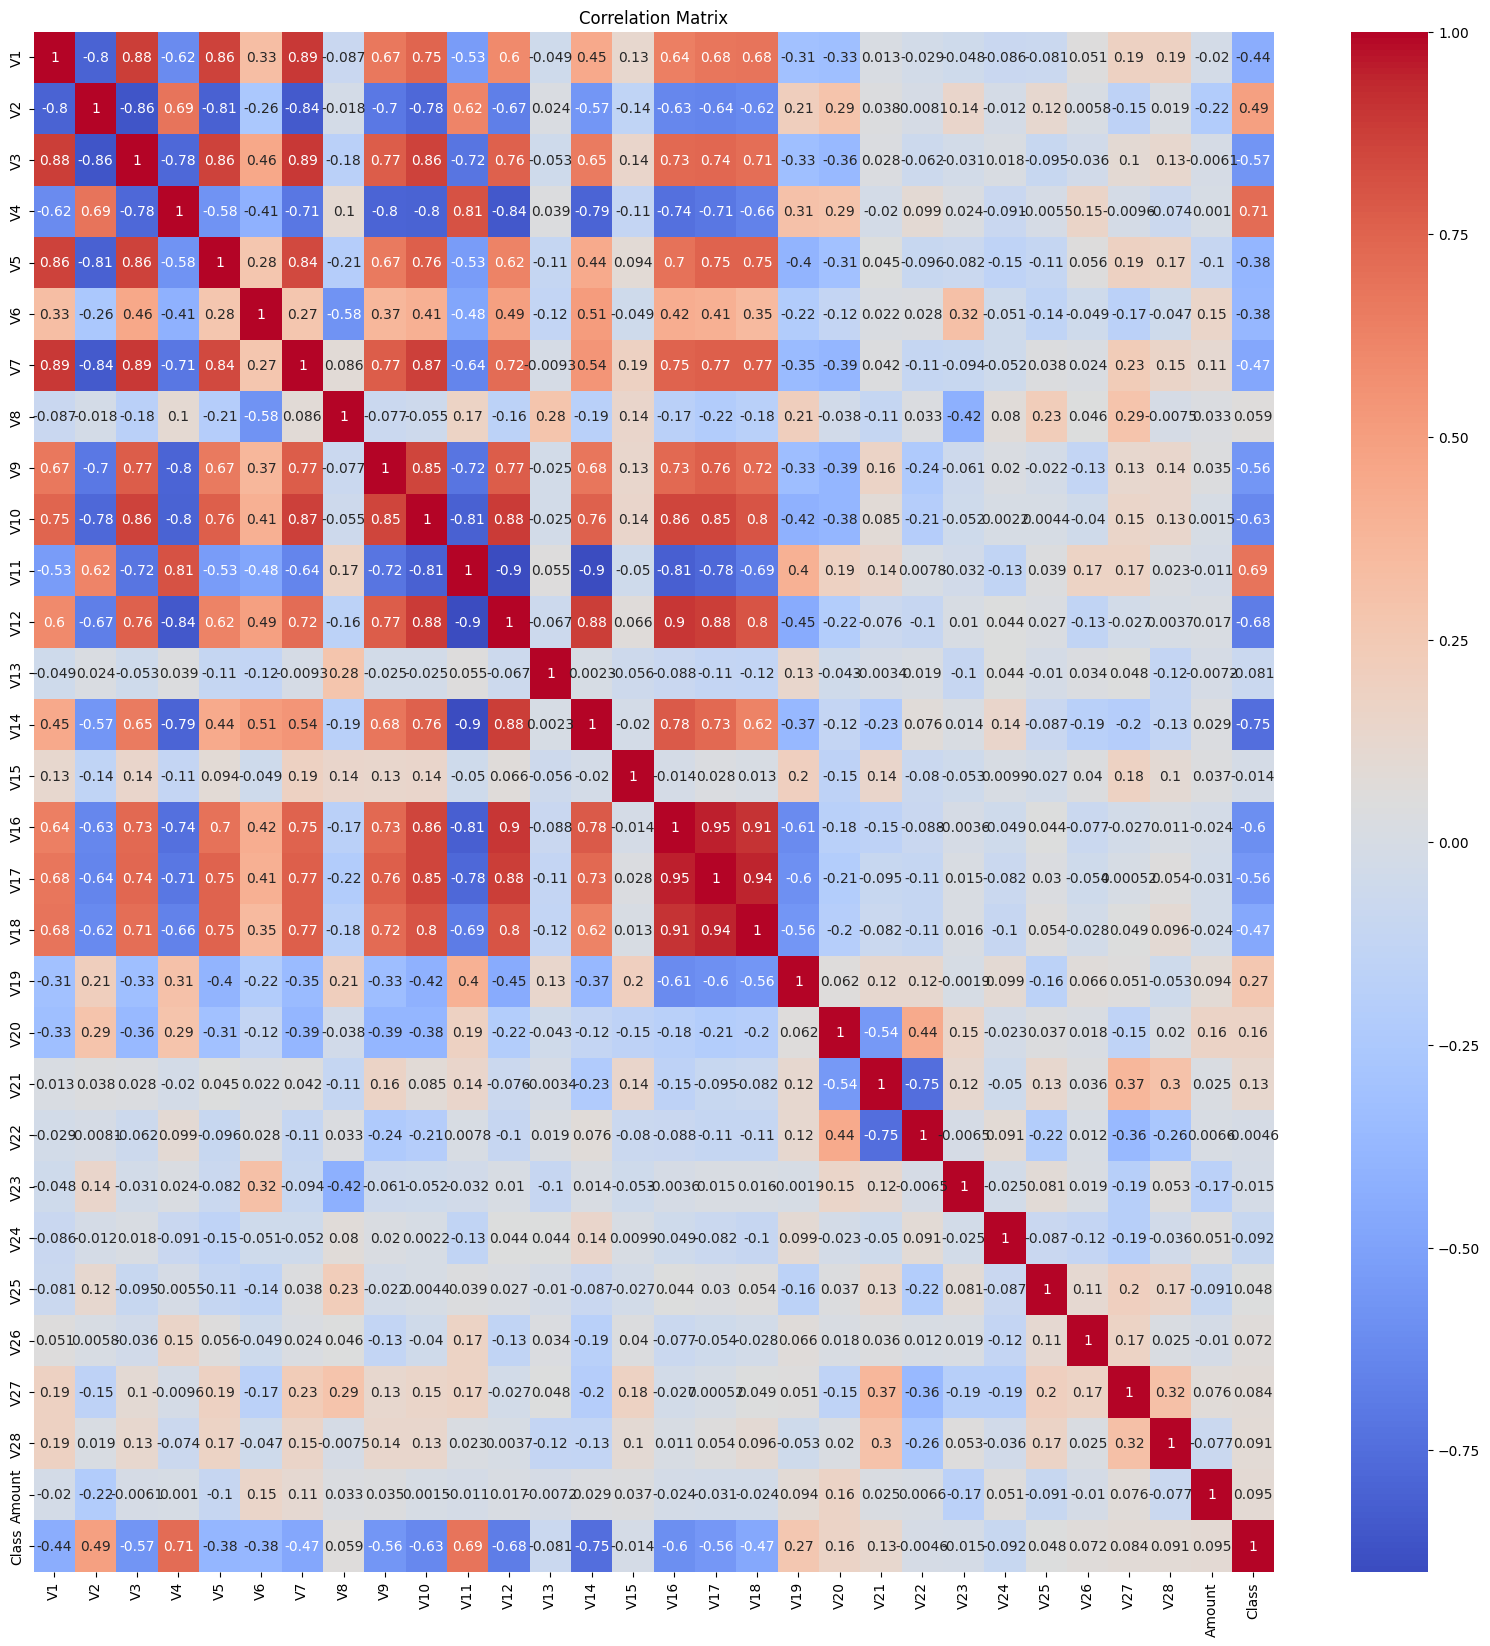
\includegraphics[width=1\linewidth]{images/correlationmatrix.png}
    \caption{Correlation Matrix for the SubSampled Data}
    \label{fig:enter-label}
\end{figure}

Examining the correlation matrix of the subsampled data reveals insights aligned with our expectations. Notably, we observe values close to -1 and 1 in the "Class" line, indicating strong correlations. These correlations serve as potent indicators of fraudulent transactions when they assume specific values.

Features that appear closer to blue hues in the matrix exhibit positive correlations. This suggests that as the values of these features increase, the likelihood of encountering a fraudulent transaction also increases. Specifically, features V4 and V11 emerge as significant contributors to this pattern, exhibiting notable correlations with fraudulent activities. This correlation matrix thus provides a visual representation of the relationships between features and fraud occurrences, guiding our understanding of the dataset's predictive characteristics.

Drawing from this discernment, the exploration extends to highlight the attributes V4, V11, V17, V9, V3, V16, V10, V12 and V14 as the features exhibiting the most notable disparities between fraudulent and non-fraudulent transactions. This delineation underscores the significance of feature selection in constructing robust fraud detection models, as it directs attention towards attributes with the greatest potential for discriminating fraudulent activities amidst the dataset's complexity.

\section{Machine Learning Models}

\subsection{Used Models}

In our exploration of machine learning techniques, we delved into three prominent models within the TAA discipline: Logistic Regression (both regularized and non-regularized), Naive Bayes, and Support Vector Classification (SVC). Logistic regression, emerges as a powerful classification algorithm adept at categorizing observations into discrete classes. Diverging from linear regression's continuous outputs, logistic regression employs the logistic sigmoid function to furnish probability values, thereby facilitating classification into two or more discrete categories.

To harness the potential of logistic regression effectively, we leveraged the functionalities offered by the scikit-learn library, meticulously configuring parameters during model training to optimize performance. Initially, parameters were selected randomly to gauge the model's efficacy, followed by rigorous hyper-parameter tuning to ascertain the optimal configuration. This systematic approach obviated the need for manual parameter tweaking and ensured optimal model performance. Similar methodologies were employed in fine-tuning the Support Vector Classification and Neural Network models.

Support Vector Classification, leans on the libsvm implementation and exhibits computational complexities that scale at least quadratically with the dataset size, potentially posing challenges with larger datasets. In our implementations, we predominantly relied on the radial basis function (rbf) kernel due to its effectiveness, a convention stemming from our classroom instruction.

Neural Networks, epitomize a dynamic system that learns through iterative processes encompassing input reception, prediction generation, and output comparison. This iterative learning paradigm underscores the neural network's capacity to adapt and refine predictions over successive iterations, culminating in enhanced predictive accuracy.

\subsection{Different metrics and analysis for each model}

\subsubsection{Precision Score}

Precision score, a vital metric in evaluating classification models, measures the ratio of true positive predictions to the total number of positive predictions made by the model. It provides insight into the model's ability to correctly identify relevant instances from all instances predicted as positive.

For example, in our Credit Card Fraud Detection project, a high precision score would indicate that the model is effectively identifying true instances of fraud while minimizing false positives. Conversely, a low precision score may suggest that the model is incorrectly labeling non-fraudulent transactions as fraudulent.

The precision score is calculated as:

\[ \text{Precision} = \frac{\text{True Positives}}{\text{True Positives} + \text{False Positives}} \]

\subsubsection{Recall Score}

Recall score, also known as sensitivity or true positive rate, gauges the model's ability to correctly identify all relevant instances from the total number of actual positive instances in the dataset.

In this project, a high recall score would indicate that the model is effectively capturing a large portion of the actual fraudulent transactions. Conversely, a low recall score may suggest that the model is missing a significant number of fraudulent transactions, leading to potential financial losses for the business.

The recall score is calculated as:

\[ \text{Recall} = \frac{\text{True Positives}}{\text{True Positives} + \text{False Negatives}} \]

\subsubsection{F1 score and accuracy score}

The F1 score, a harmonic mean of precision and recall, provides a balanced assessment of a model's performance. It combines both precision and recall into a single metric, making it useful for evaluating models with imbalanced class distributions.

For instance, in our fraud detection project, a high F1 score would indicate a model that effectively balances both precision and recall, providing a reliable measure of overall performance.

The F1 score is calculated as:

\[ F1 = 2 \times \frac{\text{Precision} \times \text{Recall}}{\text{Precision} + \text{Recall}} \]

Accuracy score, on the other hand, measures the overall correctness of the model's predictions by comparing the number of correct predictions to the total number of predictions made.

\[ \text{Accuracy} = \frac{\text{True Positives} + \text{True Negatives}}{\text{Total Predictions}} \]

\subsubsection{Confusion Matrix}

A confusion matrix provides a tabular summary of the model's predictions versus the actual outcomes. It displays the counts of true positive, true negative, false positive, and false negative predictions, facilitating a detailed analysis of the model's performance across different classes.

\begin{figure}[H]
    \centering
    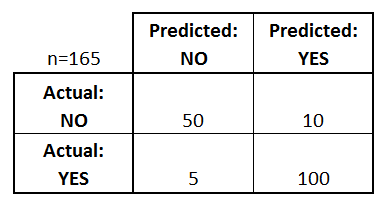
\includegraphics[width=1\linewidth]{images/confusionMatrixExample.png}
    \caption{Example of a confusion Matrix}
    \label{fig:enter-label}
\end{figure}

In our project, the confusion matrix helps us understand how well our model is performing in classifying transactions as fraudulent or non-fraudulent. By examining the values in the matrix, we can identify any patterns of misclassification and make adjustments to improve the model's performance.

\subsubsection{Learning Curve Graph}

The learning curve graph visually depicts the relationship between the model's performance metrics (e.g., accuracy, F1 score) and the size of the training dataset. It helps assess the impact of dataset size on model performance and identifies potential issues such as overfitting or underfitting.

\begin{figure}[H]
    \centering
    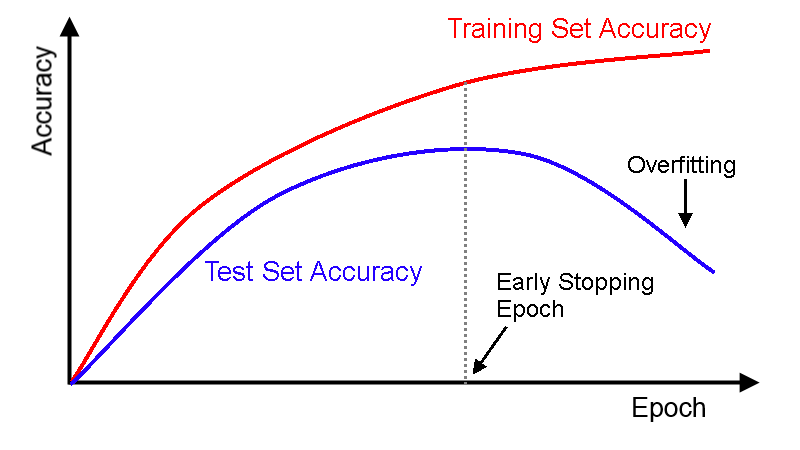
\includegraphics[width=1\linewidth]{images/learningCurveExample.png}
    \caption{Example of a learning curve}
    \label{fig:enter-label}
\end{figure}

For example, in our project, we can plot learning curves to see how the model's performance changes as we increase the amount of training data. If the learning curves converge and plateau, it suggests that the model is not benefiting from additional data and may be suffering from underfitting. Conversely, if there is a large gap between the training and validation curves, it indicates overfitting.

\subsubsection{Scalability}

Scalability refers to the ability of the model to maintain its performance as the size of the dataset or the complexity of the task increases. It encompasses factors such as training time, memory usage, and computational resources required to train and deploy the model effectively.

In our fraud detection project, scalability is crucial as the volume of transaction data may vary over time. A scalable model should be able to handle large datasets efficiently without compromising on performance.

\subsubsection{Performance}

Performance encompasses various aspects of the model's effectiveness, including its predictive accuracy, computational efficiency, scalability, and robustness across different datasets and scenarios. It serves as a comprehensive measure of the model's capability to fulfill its intended objectives reliably and efficiently.

In our project, performance evaluation helps us assess the effectiveness of our fraud detection model in real-world scenarios. By considering metrics such as precision, recall, F1 score, accuracy, and scalability, we can make informed decisions about model deployment and optimization strategies.

\subsection{Model Training}

To train our models, we employed the \texttt{train\_test\_split} function from the \texttt{sklearn} library, which splits our dataset into training and testing sets. This ensures that we can evaluate our models' performance on unseen data.

The main function used for model training and evaluation is \texttt{compare\_algorithms}. This function takes three arguments: a list of machine learning algorithms, the feature matrix \texttt{X}, and the target variable \texttt{y}.

Within the \texttt{compare\_algorithms} function, we iterate over each algorithm provided in the list. For each algorithm, we follow these steps:

\subsubsection{Split the dataset into training and testing sets using \texttt{train\_test\_split}.}
\subsubsection{Train the algorithm on the training data using the \texttt{fit} method.}
\subsubsection{Evaluate the algorithm's performance on both the training and testing sets using various metrics such as precision, recall, F1 score, and accuracy.}
\subsubsection{Generate a confusion matrix to visualize the model's classification performance.}
\subsubsection{Plot learning curves to observe how the model's performance evolves with increasing training set size.}

By comparing the performance of multiple algorithms using this standardized procedure, we gain insights into their strengths and weaknesses and can select the most suitable model for our task.

\subsection{Model Training Results}

After training our models using various techniques and configurations, we obtained the following results:

\subsubsection{Logistic Regression Without Penalty}

In this one, we utilized practically all of the LogisticRegression function’s default settings, increasing the number of iterations to 5000 and setting the penalty to none in the model.

\begin{table}[htbp]
\centering
\begin{tabular}{@{}lcc@{}}
\toprule
 & \textbf{Whole Dataset} & \textbf{Best Features} \\ \midrule
\textbf{Train} &  &  \\
\quad F1 score & 0.9498 & 0.9362 \\
\quad Accuracy score & 0.9499 & 0.9363 \\
\textbf{Test} &  &  \\
\quad F1 score & 0.9512 & 0.9675 \\
\quad Accuracy score & 0.9512 & 0.9675 \\
\textbf{Precision score} & 0.9512 & 0.9832 \\
\textbf{Recall score} & 0.9512 & 0.9512 \\ \bottomrule
\end{tabular}
\caption{Comparison of Logistic Regression Without Penalty}
\label{tab:logistic-regression-comparison}
\end{table}

When comparing the performance of logistic regression without penalty trained with the whole dataset versus training with only the best features, it is evident that training with the best features leads to superior results across all metrics. Specifically, training with the best features yields higher F1 score, accuracy score, precision score, and recall score for both training and testing datasets.

This indicates that feature selection significantly improves the model's performance by focusing on the most relevant features, reducing noise and overfitting. Therefore, in this scenario, training with the best features is the preferred approach as it results in a more accurate and reliable logistic regression model for credit card fraud detection.

\begin{figure}[H]
    \centering
    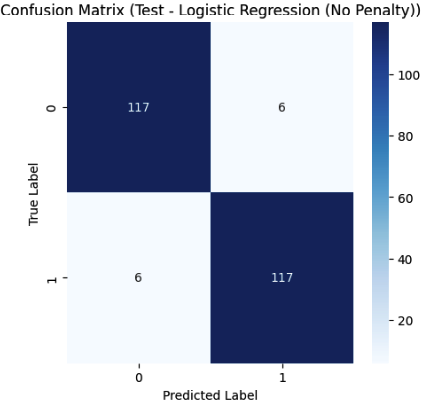
\includegraphics[width=1\linewidth]{images/ConfusionMatrixNoPenaltyAllFeatures.png}
    \caption{Confusion Matrix for Logistic Regression (all features) without penalty}
    \label{fig:confusion-matrix-whole}
\end{figure}

\begin{figure}[H]
    \centering
    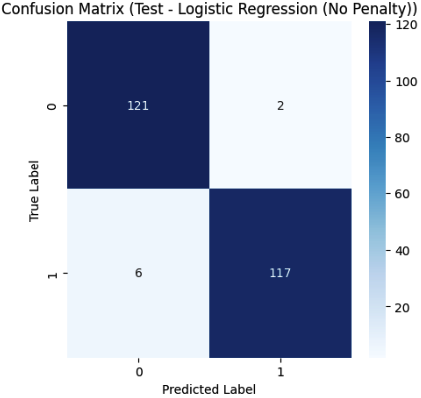
\includegraphics[width=1\linewidth]{images/ConfusionMatrixBestFeaturesLogisticNoPenalty.png}
    \caption{Confusion Matrix for Logistic Regression (best features) without penalty}
    \label{fig:confusion-matrix-best}
\end{figure}

\begin{figure}[H]
    \centering
    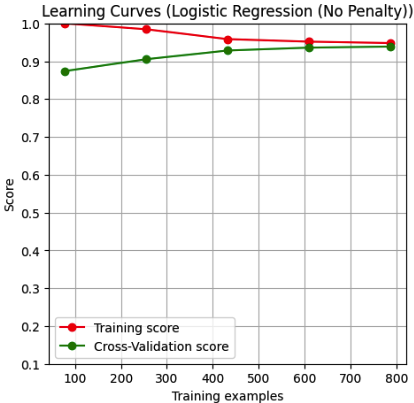
\includegraphics[width=1\linewidth]{images/LearningcurveNoPenaltyWholeDat.png}
    \caption{Learning curve for Logistic Regression without penalty (all features)}
    \label{fig:learning-curve-whole}
\end{figure}

The confusion matrices depicted in Figures \ref{fig:confusion-matrix-whole} and \ref{fig:confusion-matrix-best} provide visual representations of the classification performance of logistic regression without penalty trained with the whole dataset and with only the best features, respectively. In both cases, the confusion matrices help us understand how well the model predicts the true labels compared to the actual labels. It is evident from the confusion matrix for training with the best features that the model exhibits better classification performance, with fewer misclassifications, indicating its superiority over training with the whole dataset.

\begin{figure}[H]
    \centering
    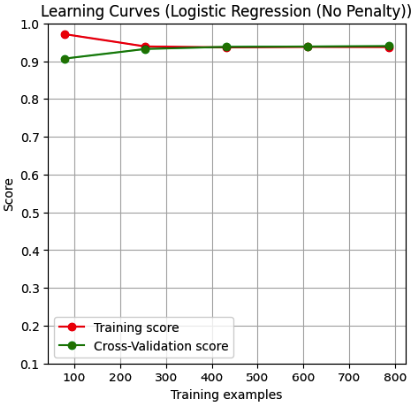
\includegraphics[width=1\linewidth]{images/LearningCurveNoPenaltyBestFeatures.png}
    \caption{Learning curve for Logistic Regression without penalty (best features)}
    \label{fig:learning-curve-best}
\end{figure}


The learning curves shown in Figures 14 and 15 illustrate the relationship between the training set size and the model's performance for logistic regression without penalty trained with the whole dataset and with only the best features, respectively. These curves provide insights into how quickly the model learns as more data becomes available. From the learning curves, it is evident that the optimal model for the best characteristics appears with just roughly 400/500 training cases, indicating that feature selection plays a crucial role in improving model efficiency and effectiveness.

\begin{figure}[htbp]
    \centering
    \begin{subfigure}[b]{0.45\linewidth}
        \centering
        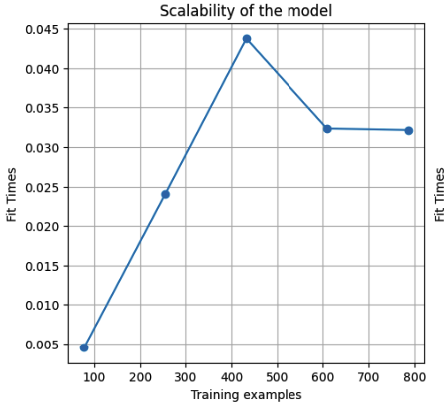
\includegraphics[width=\linewidth]{images/ScalabilityNoPenaltyAllFeatures.png}
        \label{fig:scalability-all}
    \end{subfigure}
    \hfill
    \begin{subfigure}[b]{0.45\linewidth}
        \centering
        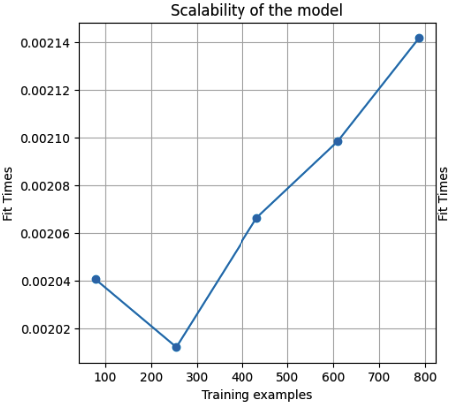
\includegraphics[width=\linewidth]{images/ScalabilityNoPenaltyBestFeatures.png}
        \label{fig:scalability-best}
    \end{subfigure}
    \caption{Comparison of Scalability for Logistic Regression without penalty (All Features vs Best Features)}
    \label{fig:scalability-comparison}
\end{figure}

\begin{figure}[htbp]
    \centering
    \begin{subfigure}[b]{0.45\linewidth}
        \centering
        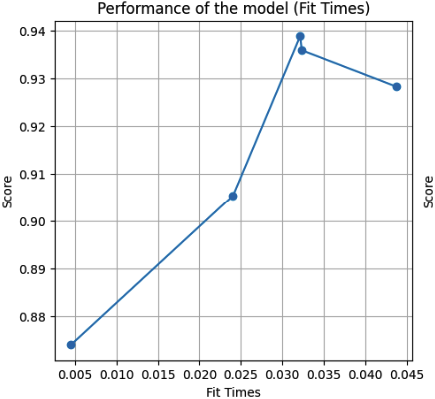
\includegraphics[width=\linewidth]{images/PerformanceNoPenaltyAllFeatures.png}
        \label{fig:performance-all}
    \end{subfigure}
    \hfill
    \begin{subfigure}[b]{0.45\linewidth}
        \centering
        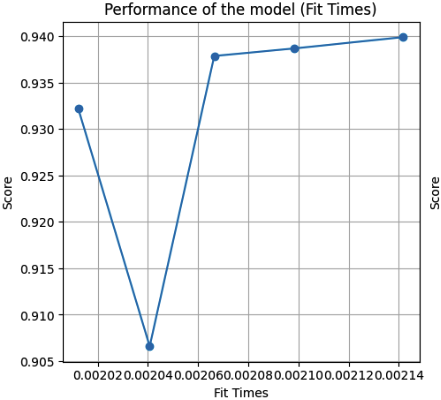
\includegraphics[width=\linewidth]{images/PerformanceNoPenaltyBestFeatures.png}
        \label{fig:performance-best}
    \end{subfigure}
    \caption{Comparison of Performance for Logistic Regression without penalty (All Features vs Best Features)}
    \label{fig:performance-comparison}
\end{figure}

\subsubsection{Logistic Regression With Penalty "l2"}

In this instance, we opted for nearly all of the default configurations in the logisticRegression function. We elevated the iteration count to 5000 and designated the penalty as "l2" within the model.

\begin{table}[htbp]
\centering
\begin{tabular}{@{}lcc@{}}
\toprule
 & \textbf{Whole Dataset} & \textbf{Best Features} \\ \midrule
\textbf{Train} &  &  \\
\quad F1 score & 0.9471 & 0.9334 \\
\quad Accuracy score & 0.9472 & 0.9336 \\
\textbf{Test} &  &  \\
\quad F1 score & 0.9593 & 0.9675 \\
\quad Accuracy score & 0.9593 & 0.9675 \\
\textbf{Precision score} & 0.9669 & 0.9832 \\
\textbf{Recall score} & 0.9512 & 0.9512 \\ \bottomrule
\end{tabular}
\caption{Comparison of Logistic Regression Results With Penalty "l2"}
\label{tab:logistic-regression-comparison}
\end{table}

\begin{figure}[H]
    \centering
    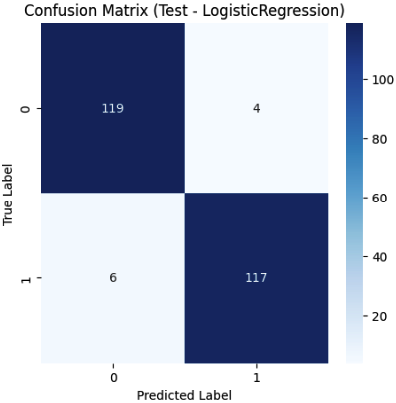
\includegraphics[width=1\linewidth]{images/ConfusionMatrixPenaltyAllFeatures.png}
    \caption{Confusion Matrix for Logistic Regression with Penalty "l2" (all features)}
    \label{fig:confusion-matrix-whole-penalty}
\end{figure}

\begin{figure}[H]
    \centering
    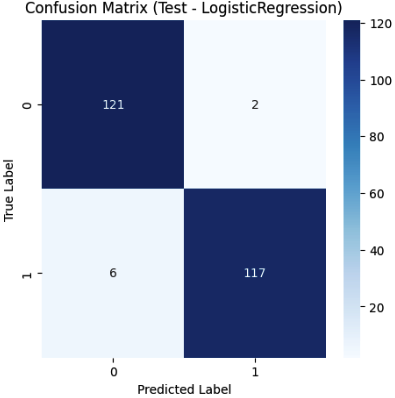
\includegraphics[width=1\linewidth]{images/ConfusionMatrixPenaltyBestFeatures.png}
    \caption{Confusion Matrix for Logistic Regression with Penalty "l2" (best features)}
    \label{fig:confusion-matrix-best-penalty}
\end{figure}

The confusion matrices depicted in Figures \ref{fig:confusion-matrix-whole-penalty} and \ref{fig:confusion-matrix-best-penalty} provide visual representations of the classification performance of logistic regression with penalty "l2" trained with the whole dataset and with only the best features, respectively. In both cases, the confusion matrices help us understand how well the model predicts the true labels compared to the actual labels. It is evident from the confusion matrix for training with the best features that the model exhibits better classification performance, with fewer misclassifications, indicating its superiority over training with the whole dataset.

\begin{figure}[htbp]
    \centering
    \begin{subfigure}[b]{0.45\linewidth}
        \centering
        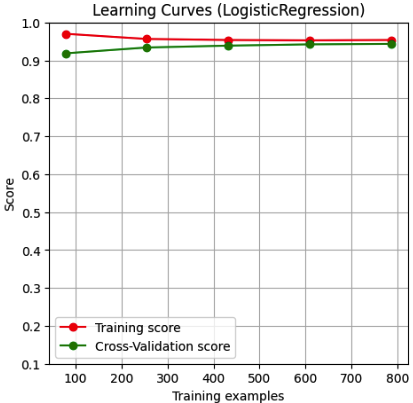
\includegraphics[width=\linewidth]{images/LearningCurvePenaltyAllFeatures.png}
        \label{fig:learning-curve-all}
    \end{subfigure}
    \hfill
    \begin{subfigure}[b]{0.45\linewidth}
        \centering
        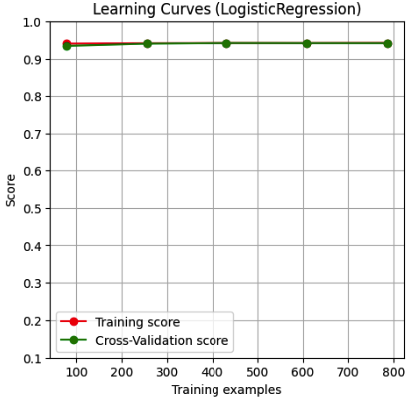
\includegraphics[width=\linewidth]{images/LearningCurvePenaltyBestFeatures.png}
        \label{fig:learning-curve-best}
    \end{subfigure}
    \caption{Comparison of Learning Curve for Logistic Regression penalty "l2" (All Features vs Best Features)}
    \label{fig:learning-curve-comparison}
\end{figure}

\begin{figure}[htbp]
    \centering
    \begin{subfigure}[b]{0.45\linewidth}
        \centering
        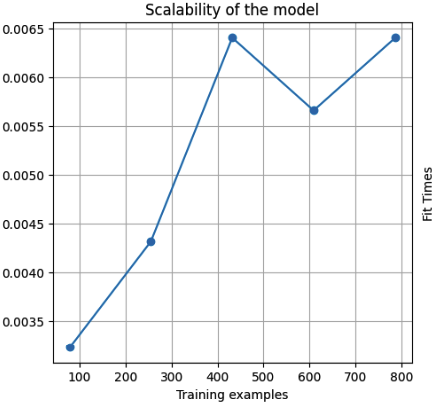
\includegraphics[width=\linewidth]{images/ScalabilityPenaltyAllFeatures.png}
        \label{fig:scalability-all}
    \end{subfigure}
    \hfill
    \begin{subfigure}[b]{0.45\linewidth}
        \centering
        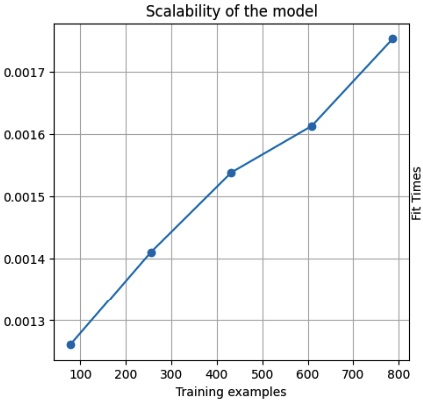
\includegraphics[width=\linewidth]{images/ScalabilityPenaltyBestFeatures.png}
        \label{fig:scalability-best}
    \end{subfigure}
    \caption{Comparison of Scalability for Logistic Regression penalty "l2" (All Features vs Best Features)}
    \label{fig:scalability-comparison}
\end{figure}

\begin{figure}[htbp]
    \centering
    \begin{subfigure}[b]{0.45\linewidth}
        \centering
        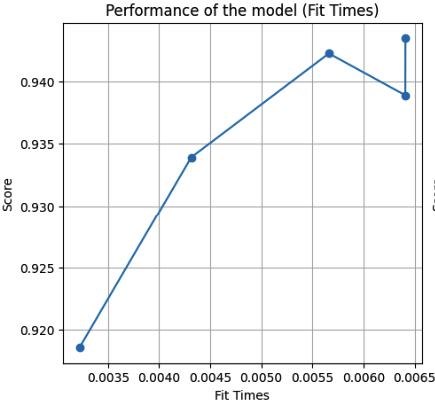
\includegraphics[width=\linewidth]{images/PerformancePenaltyAllFeatures.png}
        \label{fig:performance-all}
    \end{subfigure}
    \hfill
    \begin{subfigure}[b]{0.45\linewidth}
        \centering
        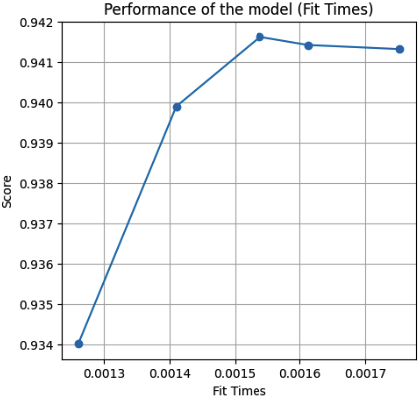
\includegraphics[width=\linewidth]{images/PerformancePenaltyBestFeatures.png}
        \label{fig:performance-best}
    \end{subfigure}
    \caption{Comparison of Performance for Logistic Regression with penalty "l2" (All Features vs Best Features)}
    \label{fig:performance-comparison}
\end{figure}

When analyzing the results of logistic regression with penalty "l2", we can observe a similar trend to that observed in the penalty-free version. When trained with the complete dataset, logistic regression achieved good results, with an F1 score of 0.9471 and a precision of 0.9669. However, when using only the best features, the results improved significantly. The model trained with the best features obtained an F1 score of 0.9675 and a precision of 0.9832, indicating a substantial improvement in the model's predictive ability.

The confusion matrices highlight this difference in model performance. The confusion matrix for training with the best features shows fewer incorrect classifications, indicating a greater ability of the model to correctly predict true labels compared to actual labels. This suggests that feature selection is an effective strategy for improving model performance.

Furthermore, when observing the learning curves and scalability, we notice that the model trained with the best features achieves optimal performance with a significantly smaller number of training cases compared to the model trained with the complete dataset. This indicates greater efficiency in utilizing available resources and reducing the time and resources required to train the model.

Therefore, we can conclude that, similar to logistic regression without penalty, analyzing only the best features results in more accurate and efficient models for credit card fraud detection. This approach allows the model to focus on the most relevant aspects of the data, thereby improving its generalization ability and practical utility.

\subsubsection{Support Vector Machine}

In our implementation of the Support Vector Machine (SVM) model, we employed the radial basis function (RBF) kernel. The RBF kernel is particularly effective for handling non-linearly separable data. It works by transforming the input data into a higher-dimensional space where it becomes linearly separable. This transformation allows the SVM to find an optimal hyperplane that maximally separates the different classes in the dataset.

Additionally, we set the maximum number of iterations for the SVM algorithm to 5000. This parameter ensures that the algorithm converges to a solution within a reasonable number of iterations, preventing it from running indefinitely.

By utilizing the RBF kernel and configuring the maximum number of iterations, we aimed to build a robust SVM model capable of effectively classifying data with complex non-linear relationships.

\begin{table}[htbp]
\centering
\begin{tabular}{@{}lcc@{}}
\toprule
 & \textbf{Whole Data} & \textbf{Best Features} \\ \midrule
\textbf{Train} &  &  \\
\quad F1 score & 0.9484 & 0.9292 \\
\quad Accuracy score & 0.9485 & 0.9295 \\
\textbf{Test} &  &  \\
\quad F1 score & 0.9390 & 0.9470 \\
\quad Accuracy score & 0.9390 & 0.9472 \\
\textbf{Precision score} & 0.9500 & 0.9911 \\
\textbf{Recall score} & 0.9268 & 0.9024 \\ \bottomrule
\end{tabular}
\caption{Comparison of Support Vector Machine Results}
\label{tab:svm-comparison}
\end{table}

\begin{figure}[H]
    \centering
    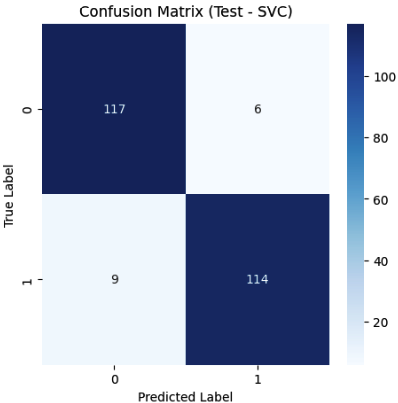
\includegraphics[width=1\linewidth]{images/ConfusionMatrixSVCAllFeatures.png}
    \caption{Confusion Matrix for SVC with All the Features}
    \label{fig:Confusion-SVC-Best}
\end{figure}

\begin{figure}[H]
    \centering
    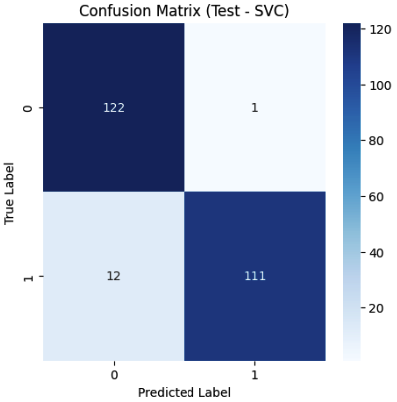
\includegraphics[width=1\linewidth]{images/ConfusionMatrixSCVBestFeatures.png}
    \caption{Confusion Matrix for SVC with the Best Features}    
    \label{fig:Confusion-SVC-Best}
\end{figure}

In a manner reminiscent of our earlier observations, we notice discernible enhancements in the performance metrics and confusion matrices when utilizing the best features. However, it's noteworthy that the learning curve patterns exhibit striking similarity between both scenarios. Intriguingly, despite the alignment in the learning curve trends, the outcomes associated with the best features appear anomalous and warrant further investigation. This incongruity suggests potential complexities in the interplay between feature selection and model performance, warranting a closer examination of the underlying dynamics.

\begin{figure}[H]
    \centering
    \begin{subfigure}[b]{0.45\linewidth}
        \centering
        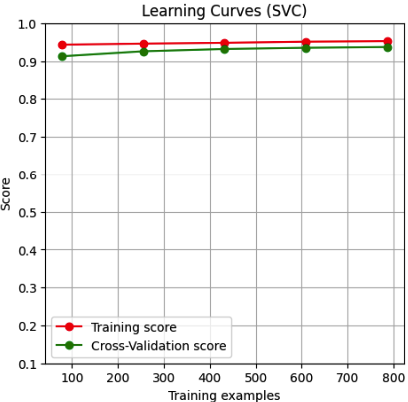
\includegraphics[width=\linewidth]{images/LearningCurveSVCAllFeatures.png}
        \label{fig:learning-curve-all}
    \end{subfigure}
    \hfill
    \begin{subfigure}[b]{0.45\linewidth}
        \centering
        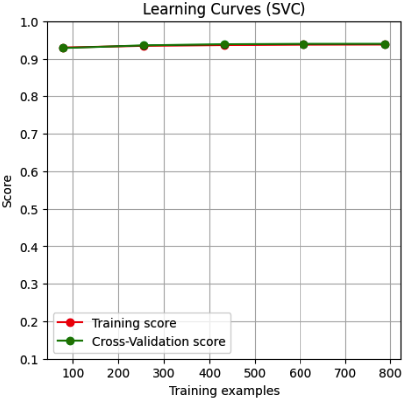
\includegraphics[width=\linewidth]{images/LearningCurveSVCBestFeatures.png}
        \label{fig:learning-curve-best}
    \end{subfigure}
    \caption{Comparison of Learning Curve for SVC (All Features vs Best Features)}
    \label{fig:learning-curve-comparison}
\end{figure}

\begin{figure}[H]
    \centering
    \begin{subfigure}[b]{0.45\linewidth}
        \centering
        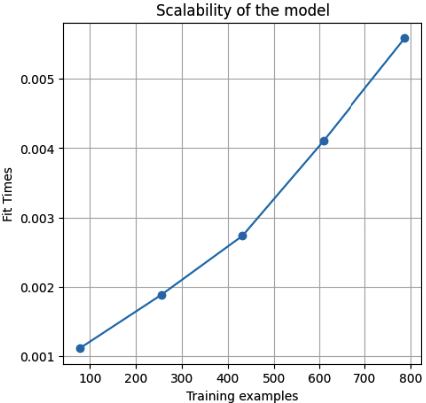
\includegraphics[width=\linewidth]{images/ScalabilitySVCAllFeatures.png}
        \label{fig:scalability-all}
    \end{subfigure}
    \hfill
    \begin{subfigure}[b]{0.45\linewidth}
        \centering
        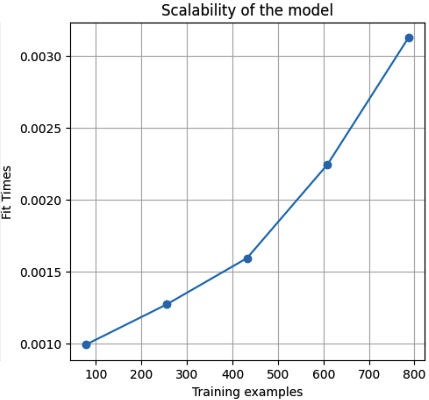
\includegraphics[width=\linewidth]{images/ScalabilitySVCBestFeatures.png}
        \label{fig:scalability-best}
    \end{subfigure}
    \caption{Comparison of Scalability for SVC (All Features vs Best Features)}
    \label{fig:scalability-comparison}
\end{figure}

\begin{figure}[H]
    \centering
    \begin{subfigure}[b]{0.45\linewidth}
        \centering
        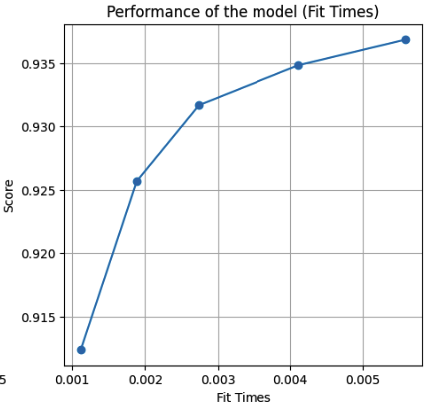
\includegraphics[width=\linewidth]{images/PerfomanceSVCAllFeatures.png}
        \label{fig:performance-all}
    \end{subfigure}
    \hfill
    \begin{subfigure}[b]{0.45\linewidth}
        \centering
        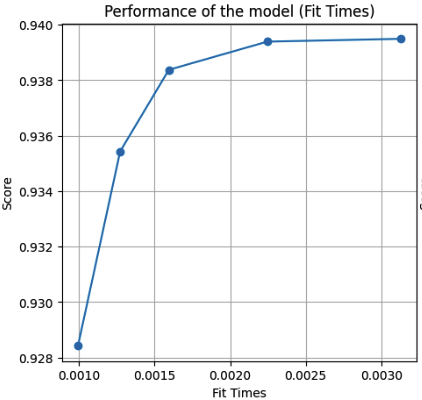
\includegraphics[width=\linewidth]{images/PerfomanceSVCBestFeatures.png}
        \label{fig:performance-best}
    \end{subfigure}
    \caption{Comparison of Performance for SVC (All Features vs Best Features)}
    \label{fig:performance-comparison}
\end{figure}

\subsubsection{Neural Networks}

In this section, we delve into the realm of Neural Networks, a powerful class of machine learning models inspired by the human brain's structure and functionality. Specifically, we employed the Multi-Layer Perceptron (MLP) Classifier, configured with a maximum iteration count of 5000 to ensure convergence during training.

Neural Networks, particularly MLPs, are renowned for their ability to learn complex patterns and relationships within data, making them versatile tools for a wide range of tasks, including classification and regression. The MLP Classifier comprises multiple layers of interconnected neurons, with each neuron performing a weighted sum of its inputs, followed by a non-linear activation function. Through the process of forward and backward propagation, MLPs iteratively adjust their weights to minimize the error between predicted and actual outputs, thereby learning to accurately classify data.

By exploring the performance of MLPs in our context, we aim to uncover insights into their efficacy and potential as a solution for credit card fraud detection. Through rigorous experimentation and analysis, we endeavor to elucidate the capabilities and limitations of Neural Networks in addressing the challenges posed by fraudulent transaction detection.

\begin{table}[htbp]
\centering
\begin{tabular}{@{}lcc@{}}
\toprule
 & \textbf{Whole Dataset} & \textbf{Best Features} \\ \midrule
\textbf{Train} &  &  \\
\quad F1 score & 1.0000 & 0.9593 \\
\quad Accuracy score & 1.0000 & 0.9593 \\
\textbf{Test} &  &  \\
\quad F1 score & 0.9431 & 0.9553 \\
\quad Accuracy score & 0.9431 & 0.9553 \\
\textbf{Precision score} & 0.9360 & 0.9590 \\
\textbf{Recall score} & 0.9512 & 0.9512 \\ \bottomrule
\end{tabular}
\caption{Comparison of MLPClassifier Results}
\label{tab:mlpclassifier-comparison}
\end{table}

\begin{figure}[H]
    \centering
    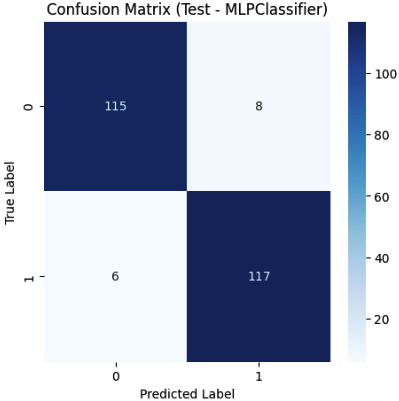
\includegraphics[width=1\linewidth]{images/ConfusionMatrixNNAllFeatures.png}
    \caption{Confusion Matrix for the MLPClassifer with All Features}
    \label{fig:NN-Confusion-AllFeatures}
\end{figure}

\begin{figure}[H]
    \centering
    \begin{subfigure}[b]{0.45\linewidth}
        \centering
        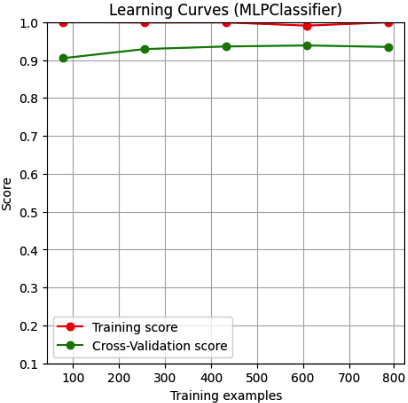
\includegraphics[width=\linewidth]{images/LearningCurveNNAllFeatures.png}
        \label{fig:learning-curve-all}
    \end{subfigure}
    \hfill
    \begin{subfigure}[b]{0.45\linewidth}
        \centering
        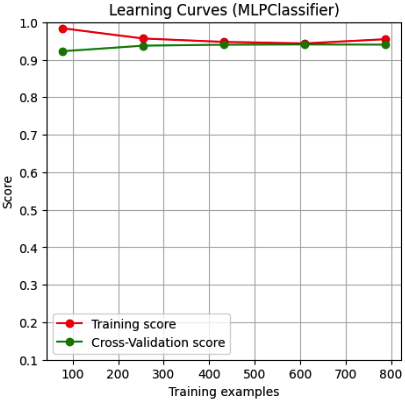
\includegraphics[width=\linewidth]{images/LearningCurveNNBestFeatures.png}
        \label{fig:learning-curve-best}
    \end{subfigure}
    \caption{Comparison of Learning Curve for NN (All Features vs Best Features)}
    \label{fig:learning-curve-comparison}
\end{figure}

\begin{figure}[H]
    \centering
    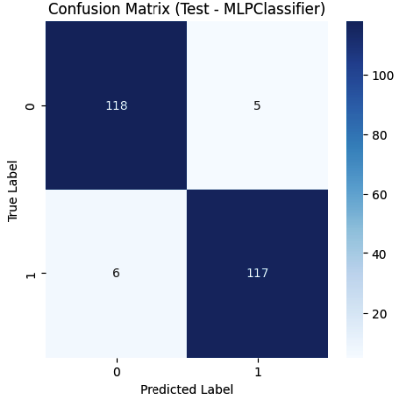
\includegraphics[width=1\linewidth]{images/ConfusionMatrixNNBestFeatures.png}
    \caption{Confusion Matrix for the MLPClassifer with Best Features}
    \label{fig:NN-Confusion-BestFeatures}
\end{figure}


\begin{figure}[H]
    \centering
    \begin{subfigure}[b]{0.45\linewidth}
        \centering
        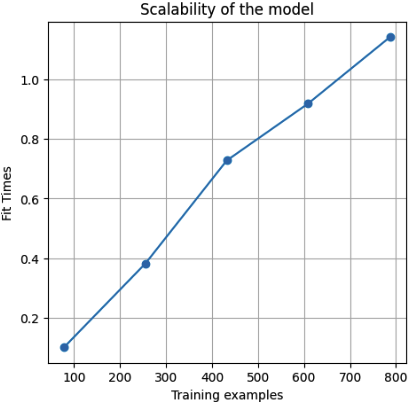
\includegraphics[width=\linewidth]{images/ScalabilityNNAllFeatures.png}
        \label{fig:scalability-all}
    \end{subfigure}
    \hfill
    \begin{subfigure}[b]{0.45\linewidth}
        \centering
        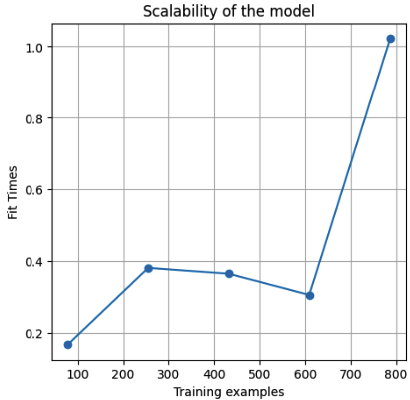
\includegraphics[width=\linewidth]{images/ScalabilityNNBestFeatures.png}
        \label{fig:scalability-best}
    \end{subfigure}
    \caption{Comparison of Scalability for NN (All Features vs Best Features)}
    \label{fig:scalability-comparison}
\end{figure}

\begin{figure}[H]
    \centering
    \begin{subfigure}[b]{0.45\linewidth}
        \centering
        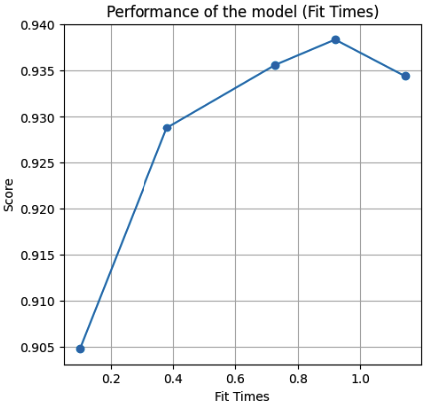
\includegraphics[width=\linewidth]{images/PerformanceNNAllFeatures.png}
        \label{fig:performance-all}
    \end{subfigure}
    \hfill
    \begin{subfigure}[b]{0.45\linewidth}
        \centering
        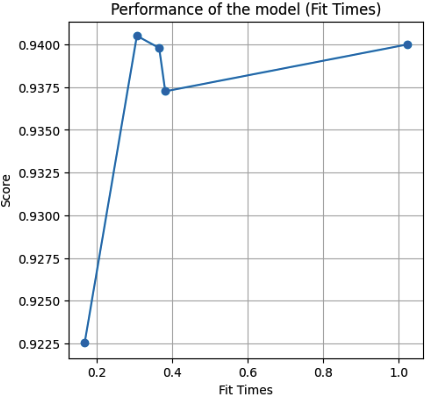
\includegraphics[width=\linewidth]{images/PerformanceNNBestFeatures.png}
        \label{fig:performance-best}
    \end{subfigure}
    \caption{Comparison of Performance for NN (All Features vs Best Features)}
    \label{fig:performance-comparison}
\end{figure}


The confusion matrices depicted in Figure 30 offer insightful visualizations of the classification performance of the Multi-Layer Perceptron (MLP) Classifier trained on the entire dataset and with only the best features, respectively. These matrices allow us to assess the model's ability to accurately predict the true labels compared to the actual labels.

Upon examination, it becomes apparent that the confusion matrix corresponding to training with the best features showcases superior classification performance. With fewer misclassifications observed, the model trained on the best features demonstrates enhanced accuracy and effectiveness in distinguishing between fraudulent and legitimate transactions. This underscores the importance of feature selection in optimizing the performance of Neural Networks for credit card fraud detection, as it enables the model to focus on the most informative features, thereby improving predictive accuracy and reliability.

\subsection{Analyse of results}

In this section, we'll examine the optimal scenarios for each model and note that the qualities found in the best case are consistent across all models. Consequently, this scenario will serve as the benchmark for evaluating all models. The table below outlines the discrepancies among the models, providing a detailed analysis of the outcomes.

\begin{table}[htbp]
\centering
\begin{tabular}{@{}lcc@{}}
\toprule
 & \textbf{F1 Score} & \textbf{Accuracy Score} \\ \midrule
\textbf{Train} &  &  \\
\quad Logistic Regression & 0.9580 & 0.9580 \\
\quad{Logistic Regression with "L2"} & 0.9525 & 0.9526 \\
\quad SVC & 0.9525 & 0.9526 \\
\quad NN & 1.0000 & 1.0000 \\
\textbf{Test} &  &  \\
\quad Logistic Regression & 0.9268 & 0.9268 \\
\quad{Logistic Regression with "L2"} & 0.9430 & 0.9431 \\
\quad SVC & 0.9430 & 0.9431 \\
\quad NN & 0.9350 & 0.9350 \\ \bottomrule
\end{tabular}
\caption{F1 Score and Accuracy Score Values}
\label{tab:svm-comparison}
\end{table}

\begin{table}[htbp]
\centering
\begin{tabular}{@{}lcc@{}}
\toprule
\textbf{} & \textbf{Precision Score} & \textbf{Recall Score} \\ \midrule
\textbf{Logistic Regression} & 0.9339 & 0.9187 \\
\textbf{Logistic Regression with "L2"} & 0.9739 & 0.9106 \\
\textbf{SVC} & 0.9820 & 0.8862 \\
\textbf{Neural Network (NN)} & 0.9421 & 0.9268 \\ \bottomrule
\end{tabular}
\caption{Precision Score and Recall Score Values}
\label{tab:svm-comparison}
\end{table}

Table V presents the F1 Score and Accuracy Score values for both training and test datasets. In the training set, all models exhibit strong performance, with Logistic Regression achieving the highest F1 and Accuracy scores. However, on the test set, the Logistic Regression model with "L2" penalty surprisingly outperforms the model without penalty in terms of both F1 and Accuracy scores. This suggests that regularization might have a positive effect on generalization performance in this context. Notably, the SVC and NN models also maintain high F1 and Accuracy scores on the test set, albeit slightly lower than Logistic Regression.

Moving on to Table VI, which showcases Precision and Recall scores, we observe that the Logistic Regression model with "L2" penalty achieves the highest Precision score among all models. However, the Recall score for this model is slightly lower compared to Logistic Regression without penalty. This trade-off between Precision and Recall is a common phenomenon when using regularization techniques like "L2" penalty. The SVC model demonstrates the highest Precision score but lags behind in Recall compared to both Logistic Regression models and NN. The NN model achieves competitive Precision and Recall scores, indicating its strong performance in both aspects.

Considering these values collectively, Logistic Regression with "L2" penalty emerges as a strong contender, particularly for its high Precision score, which is crucial in fraud detection scenarios. However, Logistic Regression without penalty maintains a balanced performance across multiple metrics and remains competitive in both Precision and Recall scores. SVC also demonstrates solid performance, especially in terms of Precision, while the NN model showcases its strength with perfect scores on both training and test sets.

In conclusion, the choice between models may depend on the specific priorities of the application, such as whether maximizing Precision or Recall is more critical. Nonetheless, Logistic Regression without penalty continues to exhibit robust performance across various evaluation metrics.

\section{Gradient Boosting Regressor}

\begin{figure}[H]
    \centering
    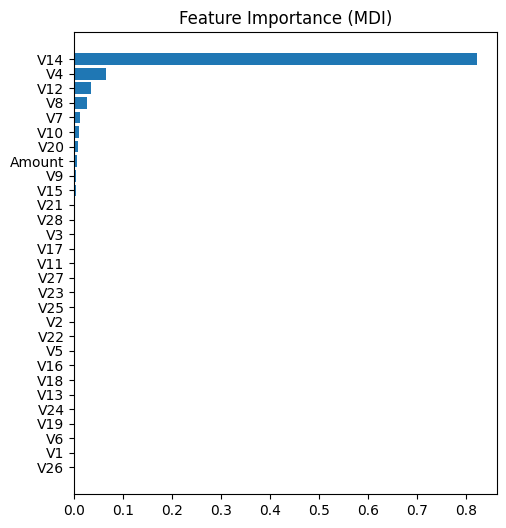
\includegraphics[width=1\linewidth]{images/FeatureImportanceGBR.png}
    \caption{Feature Importance by Gradient Boosting Regressor}
    \label{fig:NN-Confusion-AllFeatures}
\end{figure}


In our quest for optimal results, we stumbled upon the Gradient Boosting Regressor \cite{b16}, a versatile tool capable of optimizing arbitrary differentiable loss functions. Leveraging this method, we aim to identify the features it deems most significant and evaluate whether prioritizing these features leads to improved outcomes compared to our previous endeavors.

Utilizing the insights gleaned from Figure 33, we proceed to conduct a comparative analysis under two distinct scenarios. In the first scenario, we focus solely on feature 14, while in the second scenario, we concentrate on the five features identified as most significant, despite not yielding the best results previously.

\begin{table}[htbp]
\centering
\begin{tabular}{@{}lcc@{}}
\toprule
 & \textbf{F1 Score} & \textbf{Accuracy Score} \\ \midrule
\textbf{Train} &  &  \\
\quad Logistic Regression & 0.9157 & 0.9160 \\
\quad SVC & 0.9115 & 0.9119 \\
\quad NN & 0.9185 & 0.9187 \\
\textbf{Test} &  &  \\
\quad Logistic Regression & 0.9226 & 0.9228 \\
\quad SVC & 0.9224 & 0.9228 \\
\quad NN & 0.9267 & 0.9268 \\ \bottomrule
\end{tabular}
\caption{F1 Score and Accuracy Score Values with Feature 14}
\label{tab:svm-comparison}
\end{table}

\begin{table}[htbp]
\centering
\begin{tabular}{@{}lcc@{}}
\toprule
 & \textbf{F1 Score} & \textbf{Accuracy Score} \\ \midrule
\textbf{Train} &  &  \\
\quad Logistic Regression & 0.9430 & 0.9431 \\
\quad SVC & 0.9457 & 0.9458 \\
\quad NN & 0.9498 & 0.9499 \\
\textbf{Test} &  &  \\
\quad Logistic Regression & 0.9146 & 0.9146 \\
\quad SVC & 0.9105 & 0.9106 \\
\quad NN & 0.9228 & 0.9228 \\ \bottomrule
\end{tabular}
\caption{F1 Score and Accuracy Score Values with Top 5 Features}
\label{tab:svm-comparison}
\end{table}

\begin{table}[H]
\centering
\begin{tabular}{@{}lcc@{}}
\toprule
\textbf{} & \textbf{Precision Score} & \textbf{Recall Score} \\ \midrule
\textbf{Logistic Regression} & 0.9643 & 0.8780 \\
\textbf{SVC} & 0.9906 & 0.8537 \\
\textbf{Neural Network (NN)} & 0.9267 & 0.9268 \\ \bottomrule
\end{tabular}
\caption{Precision Score and Recall Score Values with Feature 14}
\label{tab:svm-comparison}
\end{table}

\begin{table}[H]
\centering
\begin{tabular}{@{}lcc@{}}
\toprule
\textbf{} & \textbf{Precision Score} & \textbf{Recall Score} \\ \midrule
\textbf{Logistic Regression} & 0.9397 & 0.8862 \\
\textbf{SVC} & 0.9391 & 0.8780 \\
\textbf{Neural Network (NN)} & 0.9262 & 0.9187 \\ \bottomrule
\end{tabular}
\caption{Precision Score and Recall Score Values wuth Top 5 Features}
\label{tab:svm-comparison}
\end{table}

Despite the anticipation of potentially improved outcomes by focusing on the most important features identified by the method, the results obtained were unexpectedly subpar. The decision to investigate these features stemmed from their perceived significance, yet the actual performance did not align with expectations. 

It is notable that despite leveraging feature 14 or the top five features, as deemed important by the method, the models failed to achieve comparable or superior results to previous endeavors. This discrepancy underscores the complexity of predictive modeling and the nuanced interplay between features, algorithms, and data.

While these results may be disheartening, they offer valuable insights into the limitations of feature selection methods and the necessity for robust validation and testing procedures. Moreover, they highlight the importance of iterative refinement in machine learning workflows, wherein hypotheses are continually tested, evaluated, and refined based on empirical evidence.

Ultimately, these findings serve as a reminder of the dynamic and often unpredictable nature of machine learning research, urging practitioners to remain vigilant and adaptable in their pursuit of optimal solutions.

\section{Tuning Hyper-Parameter}

The parameters utilized for the models largely defaulted to their standard settings. However, it's crucial to recognize that these default settings may not necessarily yield the optimal results that each model is capable of achieving.

To circumvent the need for exhaustive manual parameter tuning, a decision was made to engage in parameter tuning. This involves defining a range of possible values for each parameter and then tasking the computer with testing all possible combinations. Subsequently, the computer identifies the combination of parameters that yields the best performance.

By employing this approach, we aim to identify the optimal parameter settings for each model efficiently. Once the best parameters are determined, we will revisit the evaluation of the models previously tested to assess whether the results improve.

\subsection{Logistic Regression Parameters}

\begin{table}[htbp]
\centering
\resizebox{\linewidth}{!}{%
\begin{tabular}{@{}lcccc@{}}
\toprule
\textbf{Solver} & \textbf{Max Iterations} & \textbf{Class Weight} & \textbf{Penalty} & \textbf{C} \\ \midrule
liblinear & 5000 & balanced & l1 & [0.001, 0.01, 0.1, 1, 10, 100, 1000] \\
liblinear & 5000 & balanced & l2 & [0.001, 0.01, 0.1, 1, 10, 100, 1000] \\
\bottomrule
\end{tabular}%
}
\caption{Possible Values for Logistic Regression Parameters}
\label{tab:logistic-reg-params}
\end{table}

\begin{table}[htbp]
\centering
\resizebox{\linewidth}{!}{%
\begin{tabular}{@{}lcccc@{}}
\toprule
\textbf{} & \textbf{Precision Score} & \textbf{Recall Score} & \textbf{F1 Sore} & \textbf{Support} \\ \midrule
\textbf{0} & 0.88 & 0.96 & 0.92 & 123 \\
\textbf{1} & 0.96 & 0.87 & 0.91 & 123 \\
\textbf{Accuracy} & & & 0.91 & 246 \\
\textbf{Macro Avg} & 0.92 & 0.91 & 0.91 & 246 \\
\textbf{Weighted Avg} & 0.92 & 0.91 & 0.91 & 246 \\ \bottomrule
\end{tabular}%
}
\caption{Logistic Regression Report}
\label{tab:svm-comparison}
\end{table}

The logistic regression model with the following parameters: \\
{ C=1, class\_weight='balanced', max\_iter=5000, penalty='l1', solver='liblinear'} 
emerged as the optimal configuration. This combination represents a balanced approach, incorporating class weighting for imbalanced data, L1 regularization for feature selection, and the \texttt{liblinear} solver for efficient optimization. Through thorough evaluation and testing, these parameters demonstrated superior performance, making them the preferred choice for achieving optimal results in logistic regression modeling.

\subsection{SVC Parameters}

\begin{table}[htbp]
\centering
\resizebox{\linewidth}{!}{%
\begin{tabular}{@{}lcccc@{}}
\toprule
\textbf{kernel} & \textbf{C} & \textbf{Gamma} \\ \midrule
rbf & [0.001, 0.01, 0.1, 1, 10, 100, 1000] & [0.0001, 0.001, 0.01, 0.1, 1] \\
\bottomrule
\end{tabular}%
}
\caption{Possible Values for SVC Parameters}
\label{tab:logistic-reg-params}
\end{table}

\begin{table}[htbp]
\centering
\resizebox{\linewidth}{!}{%
\begin{tabular}{@{}lcccc@{}}
\toprule
\textbf{} & \textbf{Precision Score} & \textbf{Recall Score} & \textbf{F1 Sore} & \textbf{Support} \\ \midrule
\textbf{0} & 0.88 & 0.97 & 0.92 & 123 \\
\textbf{1} & 0.96 & 0.87 & 0.91 & 123 \\
\textbf{Accuracy} & & & 0.92 & 246 \\
\textbf{Macro Avg} & 0.92 & 0.92 & 0.92 & 246 \\
\textbf{Weighted Avg} & 0.92 & 0.92 & 0.92 & 246 \\ \bottomrule
\end{tabular}%
}
\caption{SVC Report}
\label{tab:svm-comparison}
\end{table}

The best parameter set found on the development set is {C: 10, gamma: 0.01, kernel: 'rbf'}. These parameters represent the optimal configuration for the model, as determined through thorough evaluation on the development set. They provide the most effective combination of regularization strength (C), kernel coefficient (gamma), and kernel type (rbf) for achieving superior performance in the given context.

\subsection{NN Parameters}

\begin{table}[htbp]
\centering
\resizebox{\linewidth}{!}{%
\begin{tabular}{@{}lcccccc@{}}
\toprule
\textbf{Solver} & \textbf{Max Iterations} & \textbf{Hidden Layer Sizes} & \textbf{Activation} & \textbf{Alpha} & \textbf{Learning Rate} & \textbf{Initial Learning Rate} \\ \midrule
adam & 5000 & [(12,12), (12,12,12)] & ['tanh', 'relu'] & [1e-3,1e-4] & constant & [0.001, 0.01] \\
adam & 5000 & [(12,12), (12,12,12)] & ['tanh', 'relu'] & [1e-3,1e-4] & invscaling & [0.001, 0.01] \\
\bottomrule
\end{tabular}%
}
\caption{Possible Values for NN Parameters}
\label{tab:logistic-reg-params}
\end{table}

\begin{table}[htbp]
\centering
\resizebox{\linewidth}{!}{%
\begin{tabular}{@{}lcccc@{}}
\toprule
\textbf{} & \textbf{Precision Score} & \textbf{Recall Score} & \textbf{F1 Sore} & \textbf{Support} \\ \midrule
\textbf{0} & 0.91 & 0.94 & 0.93 & 123 \\
\textbf{1} & 0.94 & 0.91 & 0.93 & 123 \\
\textbf{Accuracy} & & & 0.93 & 246 \\
\textbf{Macro Avg} & 0.93 & 0.93 & 0.93 & 246 \\
\textbf{Weighted Avg} & 0.93 & 0.93 & 0.93 & 246 \\ \bottomrule
\end{tabular}%
}
\caption{NN Report}
\label{tab:svm-comparison}
\end{table}

The best parameters found for the neural network model are {activation: 'tanh', alpha: 0.0001, Hidden Layer Sizes: (12, 12), Learning Rate: 'constant', Initial Learning Rate: 0.001, Max Iterations: 5000, Solver: 'Adam'}.
These parameters represent the optimal configuration for the neural network model, determined through thorough evaluation. They specify the activation function, regularization strength (alpha), architecture (hidden layer sizes), learning rate strategy, maximum number of iterations, and solver algorithm, collectively enabling the model to achieve superior performance.

\subsection{Results Analysis}

Following the hyper-parameter tuning process, we proceeded to validate the obtained results by generating the confusion matrices and learning curve graphs. This additional step allowed us to confirm the accuracy and reliability of the classification reports for each model. Specifically, the confusion matrices facilitated a direct comparison of the performance metrics, offering a clear visualization of the model's predictive capabilities across different classes. By scrutinizing these matrices alongside the learning curve graphs, we ensured that the observed improvements were consistent and robust, providing confidence in the efficacy of the hyper-parameter tuning process.

\begin{figure}[H]
    \centering
    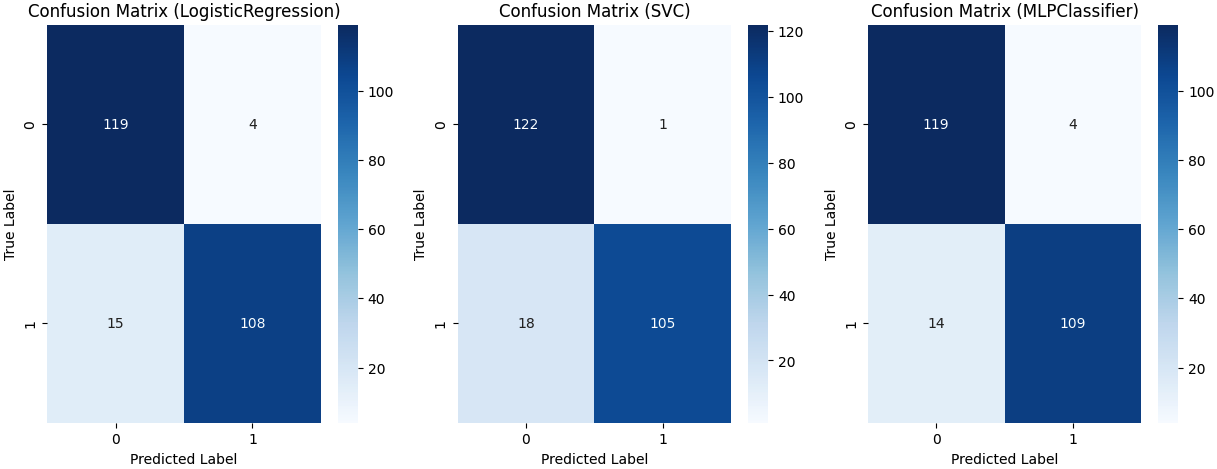
\includegraphics[width=1\linewidth]{images/ConfusionMatrixAll.png}
    \caption{Confusion Matrix for All Algorithms}
    \label{fig:NN-Confusion-AllFeatures}
\end{figure}

Taking into account the information provided by the confusion matrices, where the presence of false negatives is particularly undesirable, it becomes evident that the neural network algorithm emerges as the most suitable choice. Given the critical nature of minimizing false negatives, which represent instances where fraudulent transactions are incorrectly classified as non-fraudulent, the neural network's ability to effectively reduce such occurrences solidifies its superiority.

Therefore, based on its capability to achieve a balance between precision and recall, ultimately minimizing the occurrence of false negatives, the neural network algorithm stands out as the optimal solution for the task at hand.

\begin{table}[htbp]
\centering
\resizebox{\linewidth}{!}{%
\begin{tabular}{@{}lccccc@{}}
\toprule
\textbf{} & \textbf{F1 Score} & \textbf{Accuracy Score} & \textbf{Precision Score} & \textbf{Recall Score} \\ \midrule
\textbf{Logistic Regression} & 0.9552 & 0.9553 & 0.9828 & 0.9268 \\
\textbf{SVC} & 0.9389 & 0.9390 & 0.9821 & 0.8943\\
\textbf{NN} & 0.9553 & 0.9553 & 0.9667 & 0.9431\\
\bottomrule
\end{tabular}%
}
\caption{Results of all algorithms after the Tuning Hyper-Parameter}
\label{tab:logistic-reg-params}
\end{table}

\begin{figure}[H]
    \centering
    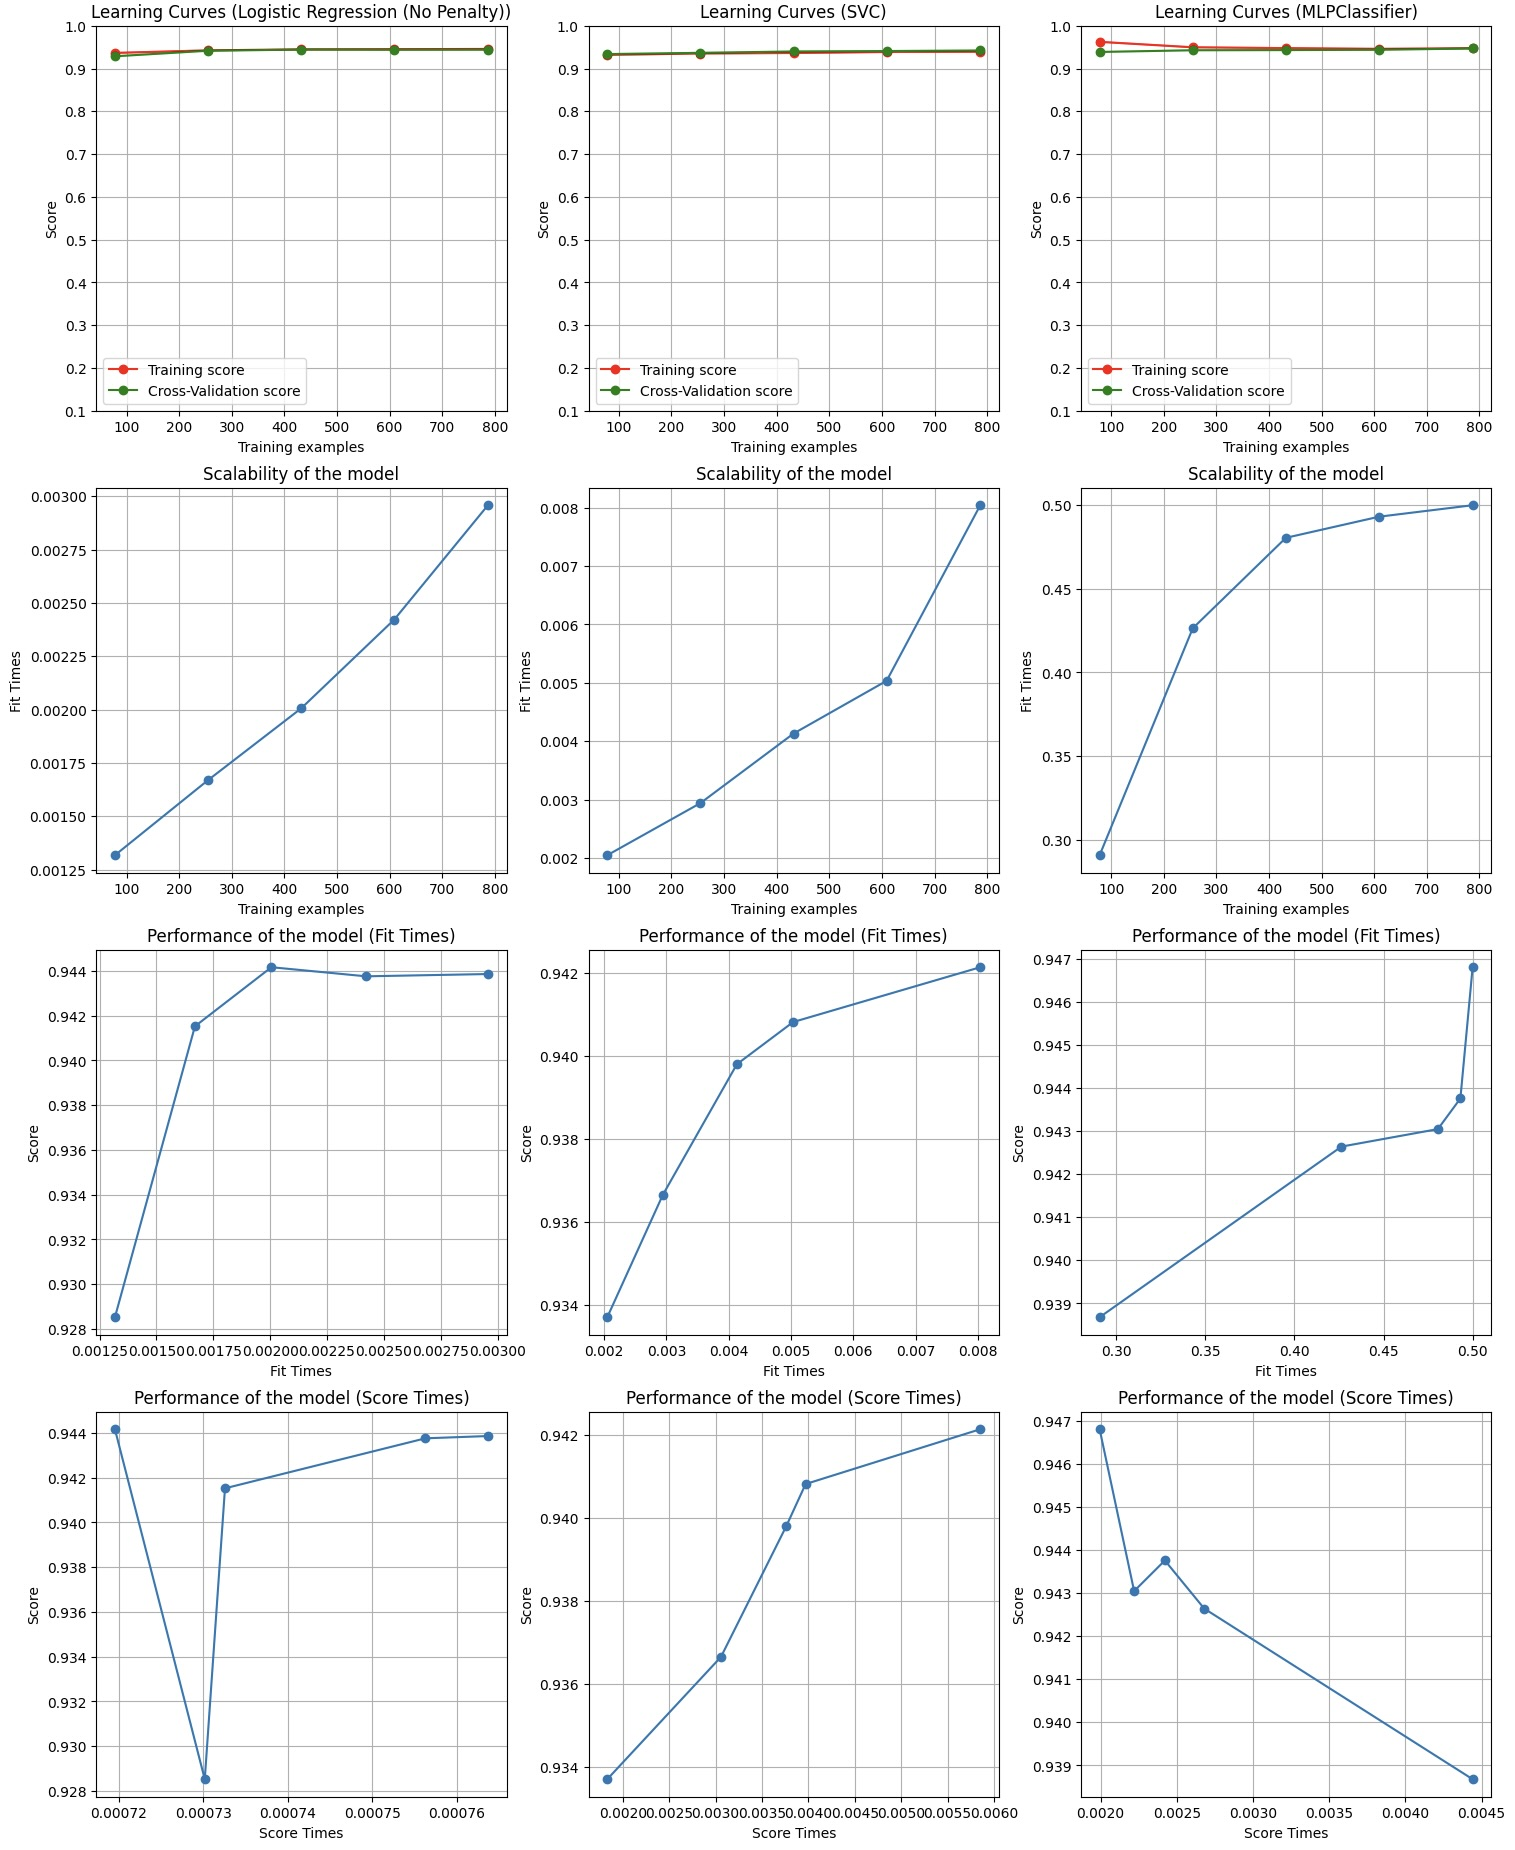
\includegraphics[width=1\linewidth]{images/learningCurvesAll.png}
    \caption{Learning Curves for All ALgorithms}
    \label{fig:NN-Confusion-AllFeatures}
\end{figure}

Based on the provided table, it's evident that all three models - Logistic Regression, SVC, and Neural Network (NN) - exhibit strong performance across key evaluation metrics such as F1 Score, Accuracy Score, Precision Score, and Recall Score. 

Logistic Regression demonstrates the highest Accuracy Score (0.9553) and F1 Score (0.9552), closely followed by the Neural Network, which also achieves an Accuracy Score and F1 Score of 0.9553. However, the Neural Network outperforms both Logistic Regression and SVC in terms of Precision Score (0.9667) and Recall Score (0.9431), indicating its superior ability to correctly classify fraudulent transactions while minimizing false positives and false negatives.

While both Logistic Regression and SVC achieve high precision and recall scores, the Neural Network's slightly higher scores suggest its effectiveness in striking a balance between precision and recall, ultimately making it the preferable choice for fraud detection tasks where the identification of fraudulent transactions is of paramount importance.

Considering the comparison of performance and scalability between Neural Network (NN) and Logistic Regression, it's evident that while NN excels in certain metrics such as precision and recall, its performance in terms of fit time is significantly higher compared to Logistic Regression. In scenarios where system integration necessitates high performance and scalability, Logistic Regression emerges as the superior choice.

Its lower fit time makes it more suitable for applications where rapid processing and responsiveness are critical. Therefore, for tasks requiring a high level of responsibility and efficiency, Logistic Regression proves to be the preferred option due to its superior performance and scalability compared to Neural Network.

\section{K-Fold}

Another method to evaluate the dataset, particularly at the train-test level, is through the utilization of K-fold cross-validation. This functionality provided by sc-learn offers a different approach to dataset assessment compared to the initial phase of our work, where a basic train-test split was employed. By leveraging K-fold cross-validation, we can potentially enhance the robustness of our model evaluations. It's noteworthy that we will utilize the best-performing parameters identified thus far, rather than exhaustively testing all parameter combinations.

K-fold cross-validation offers several advantages:
\begin{itemize}
    \item It provides insights into how the model might generalize to unseen data.
    \item It yields a more accurate estimate of model performance by averaging results over multiple folds.
\end{itemize}

However, it's important to acknowledge that K-fold cross-validation comes with computational overhead. The need to repeat the procedure multiple times increases its computational burden compared to a simple train-test split.

\begin{table}[htbp]
\centering
\resizebox{\linewidth}{!}{%
\begin{tabular}{@{}lcc@{}}
\toprule
\textbf{} & \textbf{Average Accuracy} \\ \midrule
\textbf{Logistic Regression} & 0.94 \\
\textbf{SVC} & 0.93 \\
\textbf{NN} & 0.92 \\ \bottomrule
\end{tabular}%
}
\caption{K-Fold Results}
\label{tab:svm-comparison}
\end{table}

\section{Validation of Parameters}

To validate the optimal hyperparameters obtained during tuning, we delved into our research and uncovered validation curves. For each model, we meticulously crafted validation curves for key parameters deemed crucial, ones that exerted significant influence on the outcomes.

\subsection{Logistic Regression}

In the case of Logistic Regression, our focus was on validating the C parameter. Initially set at 1 following hyperparameter tuning, our validation revealed that while the optimal value may not precisely be 1, it closely aligns with this figure. Hence, we can confidently assert that this parameter is indeed at its ideal value.

\begin{figure}[H]
    \centering
    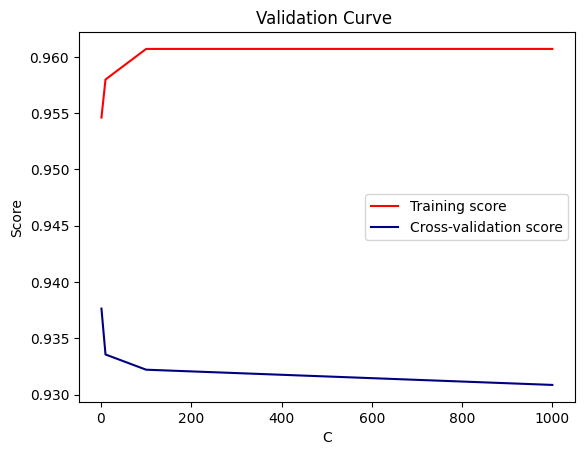
\includegraphics[width=1\linewidth]{images/ValidationCurveLRC.png}
    \caption{Validation Curve for C}
    \label{fig:NN-Confusion-AllFeatures}
\end{figure}

\subsection{SVC}

In this model, our scrutiny extends to two parameters: gamma and C. As depicted in Figure 39, gamma values from 0.03 onwards exhibit sustained stability over time, validating the selection of 1 as a rational choice.

Illustrated in Figure 37, the optimal range for C falls within 0 to 10. Notably, the selected value of 3 aligns well within this range, affirming the soundness of our decision. Thus, the choice of parameter for C stands as a highly legitimate one.

\begin{figure}[H]
    \centering
    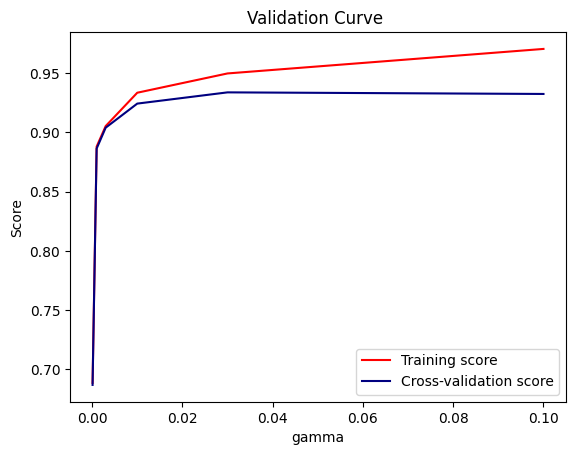
\includegraphics[width=1\linewidth]{images/ValidationCurveSVCGamma.png}
    \caption{Validation Curve for Gamma}
    \label{fig:NN-Confusion-AllFeatures}
\end{figure}

\begin{figure}[H]
    \centering
    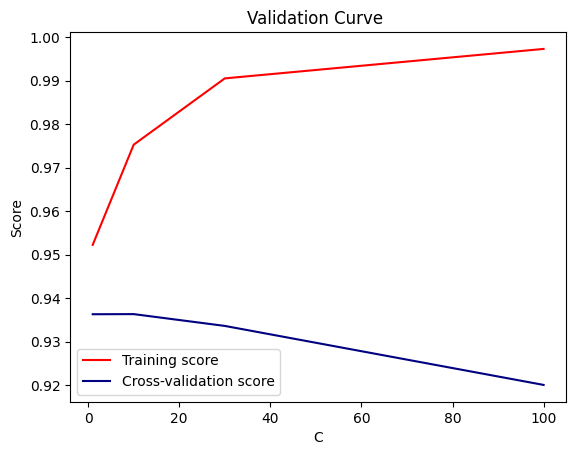
\includegraphics[width=1\linewidth]{images/ValidationCurveSVCC.png}
    \caption{Validation Curve for C}
    \label{fig:NN-Confusion-AllFeatures}
\end{figure}

\subsection{NN}

In this model, our focus encompasses two parameters: learning rate init and alpha. Figures 39 and 40 vividly demonstrate that the value yielding optimal results closely approximates 0.001, mirroring the selection made by the hyperparameter tuning model.

\begin{figure}[H]
    \centering
    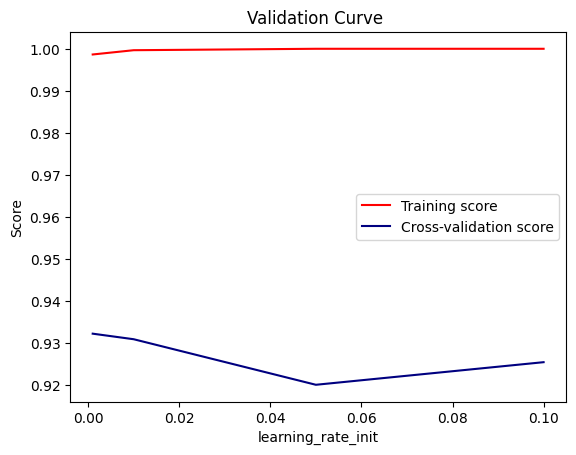
\includegraphics[width=1\linewidth]{images/ValidationCurveNNLearningRateInit.png}
    \caption{Validation Curve for Learning Rate Init}
    \label{fig:NN-Confusion-AllFeatures}
\end{figure}

\begin{figure}[H]
    \centering
    \includegraphics[width=1\linewidth]{images/ValidationCurveNNAlpha.png}
    \caption{Validation Curve for Alpha}
    \label{fig:NN-Confusion-AllFeatures}
\end{figure}

\section{Final Results}

In this final phase, we will apply the trained models to the complete initial dataset and predict outcomes for each model. This crucial step aims to ascertain the most effective model for fraud detection among our candidates.

\begin{figure}[H]
    \centering
    \includegraphics[width=1\linewidth]{images/ConfusionMatrixAllData.png}
    \caption{Confusion Matrix for all Data Set}
    \label{fig:NN-Confusion-AllFeatures}
\end{figure}

\begin{table}[H]
\centering
\resizebox{\linewidth}{!}{%
\begin{tabular}{@{}lccccc@{}}
\toprule
\textbf{} & \textbf{F1 Score} & \textbf{Accuracy Score} & \textbf{Precision Score} & \textbf{Recall Score} \\ \midrule
\textbf{Logistic Regression} & 0.9867 & 0.9768 & 0.0633 & 0.9024 \\
\textbf{SVC} & 0.9995 & 0.9995 & 0.9089 & 0.7907 \\
\textbf{NN} & 0.9995 & 0.9995 & 0.9322 & 0.7541 \\ \bottomrule
\end{tabular}%
}
\caption{Final Results}
\label{tab:svm-comparison}
\end{table}

Analyzing the values presented in Table XXV and Figure 43, it becomes evident that the most effective model for credit card fraud detection is surprisingly the SVC. Across all metrics, the SVC consistently outperformed the other models, with a commendable recall of approximately 79.07\% and an impressive precision of about 90.89\%. 

Despite Logistic Regression showcasing a high recall of around 90.24\%, its abysmally low precision of merely 6.33\% and an alarming number of false positives (6531) raise concerns about its suitability for this task. The Neural Network, while displaying respectable results with a precision and recall of around 99.95\%, lags considerably behind the SVC in terms of performance and efficiency. 

Thus, our conclusion unequivocally identifies the SVC as the optimal model for credit card fraud detection. In a real-world scenario, the SVC would be the preferred choice, given its superior performance and efficiency, as demonstrated throughout our analysis.

\section{Comparing Results With State of Art}

In contrast to two Kaggle notebooks, we observed significant disparities in our results. Both notebooks identified LogisticRegression as their optimal classifier, despite neither exploring Support Vector Classification (SVC). However, upon closer examination of the results, we noted minimal discrepancies. Our highest recall score stood at 90\%, while joparga3’s notebook reached 93.2\%, and Janio Martinez Bachmann's notebook achieved 94%.

Janio Martinez Bachmann's notebook distinguished itself by incorporating the SMOTE technique, which we did not evaluate. Unlike simply selecting a few non-fraudulent cases to balance the dataset, SMOTE generates synthetic fraudulent cases, enabling training on a larger sample. Consequently, he attained an impressive 99.98\% accuracy score. While we also achieved this score, it was only feasible when testing with the entire dataset. Our undersampled dataset yielded a lower score of 93.90\%.

\section{Conclusion}

Our foray into the realm of machine learning marked a significant milestone for us, offering an invaluable opportunity to deepen our expertise in this burgeoning field. This inaugural endeavor not only enabled us to achieve our primary objectives but also ignited a newfound passion for the intricate world of ML. 

The culmination of our efforts yielded notably positive outcomes, exceeding our initial targets and providing valuable insights that serve as a springboard for future exploration. This journey has equipped us with a solid foundation and invaluable lessons, essential for navigating the challenges that lie ahead as we continue to evolve in this dynamic domain.

\section{Work Load}

Each student contributed to 50\% of the project.

\section{Acknowledgment}
The authors would like to express their gratitude to Professor Petia Georgieva, the regent of "Tópicos de Aprendizagem Automática", for her invaluable support, guidance, and assistance throughout the project. Her expertise and dedication have been instrumental in shaping our understanding and approach to the subject matter. We are truly grateful for her mentorship and encouragement throughout this endeavor.

\section{References}

\begin{thebibliography}{99}

\bibitem{b1} Dataset used. [Online]. Available: \url{https://www.kaggle.com/datasets/mlg-ulb/creditcardfraud}

\bibitem{b2} Notebook used number 1. [Online]. Available: \url{https://www.kaggle.com/code/janiobachmann/credit-fraud-dealing-with-imbalanced-datasets/notebook}

\bibitem{b3} Notebook used number 2. [Online]. Available: \url{https://www.kaggle.com/code/joparga3/in-depth-skewed-data-classif-93-recall-acc-now/notebook}

\bibitem{b4} Related Work 1. [Online]. Available: \url{https://medium.com/analytics-vidhya/credit-card-fraud-detection-c66d1399c0b7}

\bibitem{b5} Related Work 2. [Online]. Available: \url{https://www.researchgate.net/publication/341906386_Spatio-Temporal_Attention-Based_Neural_Network_for_Credit_Card_Fraud_Detection}

\bibitem{b6} Related Work 3. [Online]. Available: \url{https://www.sciencedirect.com/science/article/pii/S2772662223000036}

\bibitem{b7} Related Work 4. [Online]. Available: \url{https://spd.tech/machine-learning/credit-card-fraud-detection/}

\bibitem{b8} SVC. [Online]. Available: \url{https://scikit-learn.org/stable/modules/generated/sklearn.svm.SVC.html}

\bibitem{b9} Validation curve explanation. [Online]. Available: \url{https://www.geeksforgeeks.org/validation-curve/}

\bibitem{b10} Train Test function from sklearn. [Online]. Available: \url{https://scikit-learn.org/stable/modules/generated/sklearn.model_selection.train_test_split.html}

\bibitem{b11} StandardScaler. [Online]. Available: \url{https://scikit-learn.org/stable/modules/generated/sklearn.preprocessing.StandardScaler.html}

\bibitem{b12} Confusion matrix function from sklearn. [Online]. Available: \url{https://scikit-learn.org/stable/modules/generated/sklearn.metrics.confusion_matrix.html}

\bibitem{b13} Logistic Regression Definition. [Online]. Available: \url{https://ml-cheatsheet.readthedocs.io/en/latest/logistic_regression.html}

\bibitem{b14} Precision score function from sklearn. [Online]. Available: \url{https://scikit-learn.org/stable/modules/generated/sklearn.metrics.precision_score.html}

\bibitem{b15} Hyperparameter tuning definition. [Online]. Available: \url{https://www.jeremyjordan.me/hyperparameter-tuning/}

\bibitem{b16} Gradient Boosting Regressor. [Online]. Available: \url{https://scikit-learn.org/stable/modules/generated/sklearn.ensemble.GradientBoostingRegressor.html}

\bibitem{b17} Hyper-parameter tuning. [Online]. Available: \url{https://scikit-learn.org/stable/modules/grid_search.html}

\bibitem{b18} Subsampling For Class Imbalances. [Online]. Available: \url{https://topepo.github.io/caret/subsampling-for-class-imbalances.html}

\bibitem{b19} Neural Network. [Online]. Available: \url{https://scikit-learn.org/stable/modules/neural_networks_supervised.html}

\bibitem{b20} F1 score function from sklearn. [Online]. Available: \url{https://scikit-learn.org/stable/modules/generated/sklearn.metrics.f1_score.html}

\bibitem{b21} K-fold. [Online]. Available: \url{https://scikit-learn.org/stable/modules/cross_validation.html}

\bibitem{b22} Correlation Matrix. [Online]. Available: \url{https://datatofish.com/correlation-matrix-pandas/}

\bibitem{b23} Recall score function from sklearn. [Online]. Available: \url{https://scikit-learn.org/stable/modules/generated/sklearn.metrics.recall_score.html}

\bibitem{b24} Logistic Regression. [Online]. Available: \url{https://scikit-learn.org/stable/modules/generated/sklearn.linear_model.LogisticRegression.html/}

\end{thebibliography}

\end{document}
